% Options for packages loaded elsewhere
% Options for packages loaded elsewhere
\PassOptionsToPackage{unicode}{hyperref}
\PassOptionsToPackage{hyphens}{url}
\PassOptionsToPackage{dvipsnames,svgnames,x11names}{xcolor}
%
\documentclass[
  letterpaper,
  DIV=11,
  numbers=noendperiod]{scrartcl}
\usepackage{xcolor}
\usepackage[paperwidth=210mm,paperheight=297mm,margin=1mm,noheadfoot]{geometry}
\usepackage{amsmath,amssymb}
\setcounter{secnumdepth}{5}
\usepackage{iftex}
\ifPDFTeX
  \usepackage[T1]{fontenc}
  \usepackage[utf8]{inputenc}
  \usepackage{textcomp} % provide euro and other symbols
\else % if luatex or xetex
  \usepackage{unicode-math} % this also loads fontspec
  \defaultfontfeatures{Scale=MatchLowercase}
  \defaultfontfeatures[\rmfamily]{Ligatures=TeX,Scale=1}
\fi
\usepackage{lmodern}
\ifPDFTeX\else
  % xetex/luatex font selection
\fi
% Use upquote if available, for straight quotes in verbatim environments
\IfFileExists{upquote.sty}{\usepackage{upquote}}{}
\IfFileExists{microtype.sty}{% use microtype if available
  \usepackage[]{microtype}
  \UseMicrotypeSet[protrusion]{basicmath} % disable protrusion for tt fonts
}{}
\makeatletter
\@ifundefined{KOMAClassName}{% if non-KOMA class
  \IfFileExists{parskip.sty}{%
    \usepackage{parskip}
  }{% else
    \setlength{\parindent}{0pt}
    \setlength{\parskip}{6pt plus 2pt minus 1pt}}
}{% if KOMA class
  \KOMAoptions{parskip=half}}
\makeatother
% Make \paragraph and \subparagraph free-standing
\makeatletter
\ifx\paragraph\undefined\else
  \let\oldparagraph\paragraph
  \renewcommand{\paragraph}{
    \@ifstar
      \xxxParagraphStar
      \xxxParagraphNoStar
  }
  \newcommand{\xxxParagraphStar}[1]{\oldparagraph*{#1}\mbox{}}
  \newcommand{\xxxParagraphNoStar}[1]{\oldparagraph{#1}\mbox{}}
\fi
\ifx\subparagraph\undefined\else
  \let\oldsubparagraph\subparagraph
  \renewcommand{\subparagraph}{
    \@ifstar
      \xxxSubParagraphStar
      \xxxSubParagraphNoStar
  }
  \newcommand{\xxxSubParagraphStar}[1]{\oldsubparagraph*{#1}\mbox{}}
  \newcommand{\xxxSubParagraphNoStar}[1]{\oldsubparagraph{#1}\mbox{}}
\fi
\makeatother


\usepackage{longtable,booktabs,array}
\usepackage{calc} % for calculating minipage widths
% Correct order of tables after \paragraph or \subparagraph
\usepackage{etoolbox}
\makeatletter
\patchcmd\longtable{\par}{\if@noskipsec\mbox{}\fi\par}{}{}
\makeatother
% Allow footnotes in longtable head/foot
\IfFileExists{footnotehyper.sty}{\usepackage{footnotehyper}}{\usepackage{footnote}}
\makesavenoteenv{longtable}
\usepackage{graphicx}
\makeatletter
\newsavebox\pandoc@box
\newcommand*\pandocbounded[1]{% scales image to fit in text height/width
  \sbox\pandoc@box{#1}%
  \Gscale@div\@tempa{\textheight}{\dimexpr\ht\pandoc@box+\dp\pandoc@box\relax}%
  \Gscale@div\@tempb{\linewidth}{\wd\pandoc@box}%
  \ifdim\@tempb\p@<\@tempa\p@\let\@tempa\@tempb\fi% select the smaller of both
  \ifdim\@tempa\p@<\p@\scalebox{\@tempa}{\usebox\pandoc@box}%
  \else\usebox{\pandoc@box}%
  \fi%
}
% Set default figure placement to htbp
\def\fps@figure{htbp}
\makeatother





\setlength{\emergencystretch}{3em} % prevent overfull lines

\providecommand{\tightlist}{%
  \setlength{\itemsep}{0pt}\setlength{\parskip}{0pt}}



 


\KOMAoption{captions}{tableheading}
\makeatletter
\@ifpackageloaded{caption}{}{\usepackage{caption}}
\AtBeginDocument{%
\ifdefined\contentsname
  \renewcommand*\contentsname{Table of contents}
\else
  \newcommand\contentsname{Table of contents}
\fi
\ifdefined\listfigurename
  \renewcommand*\listfigurename{List of Figures}
\else
  \newcommand\listfigurename{List of Figures}
\fi
\ifdefined\listtablename
  \renewcommand*\listtablename{List of Tables}
\else
  \newcommand\listtablename{List of Tables}
\fi
\ifdefined\figurename
  \renewcommand*\figurename{Figure}
\else
  \newcommand\figurename{Figure}
\fi
\ifdefined\tablename
  \renewcommand*\tablename{Table}
\else
  \newcommand\tablename{Table}
\fi
}
\@ifpackageloaded{float}{}{\usepackage{float}}
\floatstyle{ruled}
\@ifundefined{c@chapter}{\newfloat{codelisting}{h}{lop}}{\newfloat{codelisting}{h}{lop}[chapter]}
\floatname{codelisting}{Listing}
\newcommand*\listoflistings{\listof{codelisting}{List of Listings}}
\makeatother
\makeatletter
\makeatother
\makeatletter
\@ifpackageloaded{caption}{}{\usepackage{caption}}
\@ifpackageloaded{subcaption}{}{\usepackage{subcaption}}
\makeatother
\usepackage{bookmark}
\IfFileExists{xurl.sty}{\usepackage{xurl}}{} % add URL line breaks if available
\urlstyle{same}
\hypersetup{
  pdftitle={Annexes 2 : figures},
  colorlinks=true,
  linkcolor={blue},
  filecolor={Maroon},
  citecolor={Blue},
  urlcolor={Blue},
  pdfcreator={LaTeX via pandoc}}


\title{Annexes 2 : figures}
\author{}
\date{}
\begin{document}
\maketitle

\renewcommand*\contentsname{Sommaire}
{
\hypersetup{linkcolor=}
\setcounter{tocdepth}{2}
\tableofcontents
}

\newpage

\section{Nombre moyen de jour de pluie (seuil 1 mm/j) par année
hydrologique issu de Données journalières
(1959-2022)}\label{nombre-moyen-de-jour-de-pluie-seuil-1-mmj-par-annuxe9e-hydrologique-issu-de-donnuxe9es-journaliuxe8res-1959-2022}

Saturation des 0.1\% valeurs les plus extrêmes.

\begin{longtable*}{m{2.0cm}m{7.9cm}m{7.9cm}m{1cm}}
 & \centering  & \centering  & \tabularnewline
\centering \textbf{HYDRO} \\[0.2em] \begin{tabular}{r@{\hspace{0.2em}}l}$r$  & $= 0.95$ \\ ME   & $= 6.35$ \\ $n$  & $= 1583$ \\ \end{tabular} & \centering 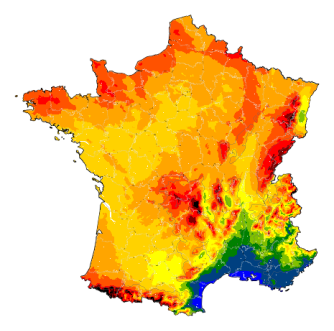
\includegraphics[width=7.9cm]{../outputs/maps/stats_numday/quotidien/compare_1/sat_99.9/hydro/mod_norast.pdf} & \centering 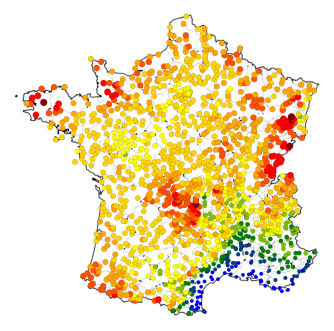
\includegraphics[width=7.9cm]{../outputs/maps/stats_numday/quotidien/compare_1/sat_99.9/hydro/obs_norast.pdf} & \centering \includegraphics[width=1cm]{../outputs/maps/stats_numday/quotidien/compare_1/sat_99.9/legend.pdf} \tabularnewline
\end{longtable*}

\section{Cumul moyen des précipitations par année
hydrologique}\label{cumul-moyen-des-pruxe9cipitations-par-annuxe9e-hydrologique}

Saturation des 0.5\% valeurs les plus extrêmes.

\subsection{Données journalières
(1959-2022)}\label{donnuxe9es-journaliuxe8res-1959-2022}

\begin{longtable*}{m{2.0cm}m{7.9cm}m{7.9cm}m{1cm}}
 & \centering  & \centering  & \tabularnewline
\centering \textbf{HYDRO} \\[0.2em] \begin{tabular}{r@{\hspace{0.2em}}l}$r$  & $= 0.94$ \\ ME   & $= 0.03$ \\ $n$  & $= 1583$ \\ \end{tabular} & \centering 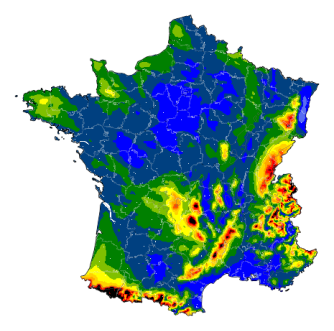
\includegraphics[width=7.9cm]{../outputs/maps/stats_mean/quotidien/compare_1/sat_99.5/hydro/mod_norast.pdf} & \centering 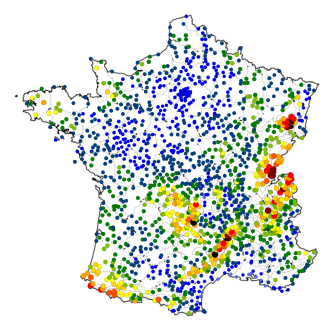
\includegraphics[width=7.9cm]{../outputs/maps/stats_mean/quotidien/compare_1/sat_99.5/hydro/obs_norast.pdf} & \centering \includegraphics[width=1cm]{../outputs/maps/stats_mean/quotidien/compare_1/sat_99.5/legend.pdf} \tabularnewline
\end{longtable*}

\subsection{Données horaires
(1990-2022)}\label{donnuxe9es-horaires-1990-2022}

\begin{longtable*}{m{2.0cm}m{7.9cm}m{7.9cm}m{1cm}}
 & \centering  & \centering  & \tabularnewline
\centering \textbf{HYDRO} \\[0.2em] \begin{tabular}{r@{\hspace{0.2em}}l}$r$  & $= 0.94$ \\ ME   & $= 0.00$ \\ $n$  & $= 574$ \\ \end{tabular} & \centering 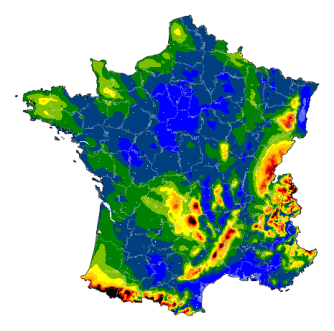
\includegraphics[width=7.9cm]{../outputs/maps/stats_mean/horaire/compare_1/sat_99.5/hydro/mod_norast.pdf} & \centering 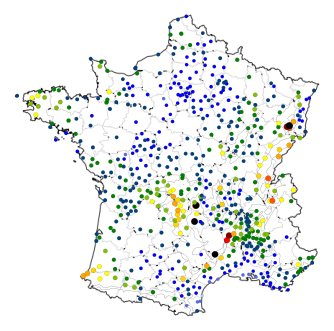
\includegraphics[width=7.9cm]{../outputs/maps/stats_mean/horaire/compare_1/sat_99.5/hydro/obs_norast.pdf} & \centering \includegraphics[width=1cm]{../outputs/maps/stats_mean/horaire/compare_1/sat_99.5/legend.pdf} \tabularnewline
\end{longtable*}

\section{Moyenne des maxima des
précipitations}\label{moyenne-des-maxima-des-pruxe9cipitations}

Saturation des 0.5\% valeurs les plus extrêmes.

\subsection{Données journalières
(1959-2022)}\label{donnuxe9es-journaliuxe8res-1959-2022-1}

\subsubsection{Par année hydrologique}\label{par-annuxe9e-hydrologique}

\begin{longtable*}{m{2.0cm}m{7.9cm}m{7.9cm}m{1cm}}
 & \centering  & \centering  & \tabularnewline
\centering \textbf{HYDRO} \\[0.2em] \begin{tabular}{r@{\hspace{0.2em}}l}$r$  & $= 0.96$ \\ ME   & $= -1.18$ \\ $n$  & $= 1583$ \\ \end{tabular} & \centering 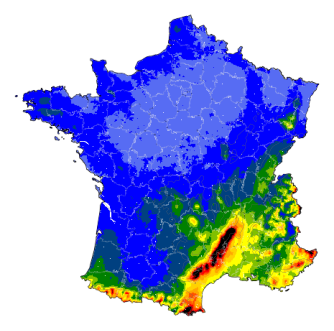
\includegraphics[width=7.9cm]{../outputs/maps/stats_mean-max/quotidien/compare_1/sat_99.5/hydro/mod_norast.pdf} & \centering 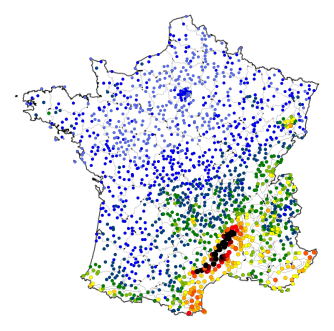
\includegraphics[width=7.9cm]{../outputs/maps/stats_mean-max/quotidien/compare_1/sat_99.5/hydro/obs_norast.pdf} & \centering \includegraphics[width=1cm]{../outputs/maps/stats_mean-max/quotidien/compare_1/sat_99.5/legend.pdf} \tabularnewline
\end{longtable*}

\subsubsection{Par saison}\label{par-saison}

\begin{longtable*}{m{2.0cm}m{7.9cm}m{7.9cm}m{1cm}}
 & \centering  & \centering  & \tabularnewline
\centering \textbf{SON} \\[0.2em] \begin{tabular}{r@{\hspace{0.2em}}l}$r$  & $= 0.97$ \\ ME   & $= -0.41$ \\ $n$  & $= 1664$ \\ \end{tabular} & \centering 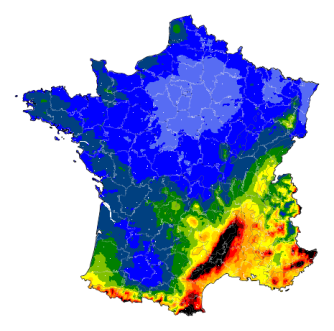
\includegraphics[width=7.9cm]{../outputs/maps/stats_mean-max/quotidien/compare_4/sat_99.5/son/mod_norast.pdf} & \centering 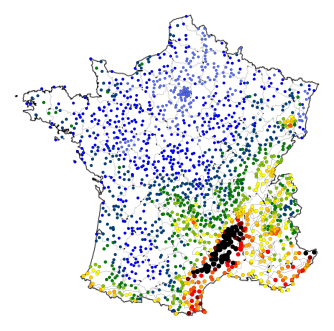
\includegraphics[width=7.9cm]{../outputs/maps/stats_mean-max/quotidien/compare_4/sat_99.5/son/obs_norast.pdf} & \centering \includegraphics[width=1cm]{../outputs/maps/stats_mean-max/quotidien/compare_4/sat_99.5/legend.pdf} \tabularnewline
\centering \textbf{DJF} \\[0.2em] \begin{tabular}{r@{\hspace{0.2em}}l}$r$  & $= 0.96$ \\ ME   & $= 0.01$ \\ $n$  & $= 1603$ \\ \end{tabular} & \centering 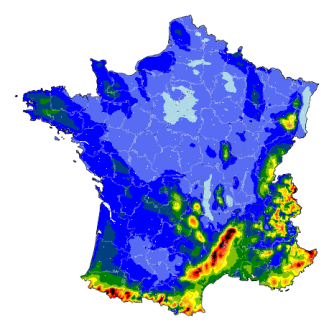
\includegraphics[width=7.9cm]{../outputs/maps/stats_mean-max/quotidien/compare_4/sat_99.5/djf/mod_norast.pdf} & \centering 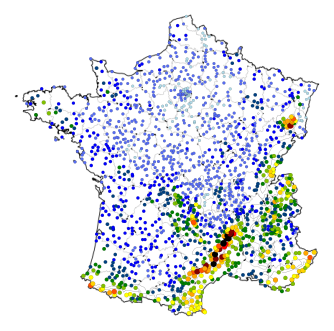
\includegraphics[width=7.9cm]{../outputs/maps/stats_mean-max/quotidien/compare_4/sat_99.5/djf/obs_norast.pdf} & \centering \includegraphics[width=1cm]{../outputs/maps/stats_mean-max/quotidien/compare_4/sat_99.5/legend.pdf} \tabularnewline
\centering \textbf{MAM} \\[0.2em] \begin{tabular}{r@{\hspace{0.2em}}l}$r$  & $= 0.95$ \\ ME   & $= -0.02$ \\ $n$  & $= 1650$ \\ \end{tabular} & \centering 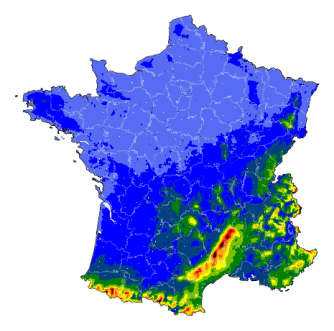
\includegraphics[width=7.9cm]{../outputs/maps/stats_mean-max/quotidien/compare_4/sat_99.5/mam/mod_norast.pdf} & \centering 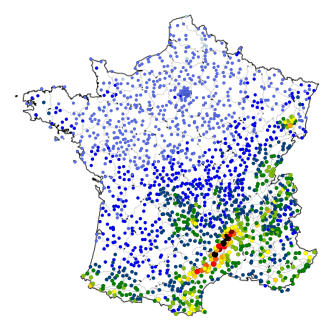
\includegraphics[width=7.9cm]{../outputs/maps/stats_mean-max/quotidien/compare_4/sat_99.5/mam/obs_norast.pdf} & \centering \includegraphics[width=1cm]{../outputs/maps/stats_mean-max/quotidien/compare_4/sat_99.5/legend.pdf} \tabularnewline
\centering \textbf{JJA} \\[0.2em] \begin{tabular}{r@{\hspace{0.2em}}l}$r$  & $= 0.87$ \\ ME   & $= -3.05$ \\ $n$  & $= 1640$ \\ \end{tabular} & \centering 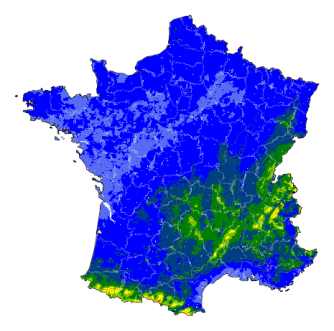
\includegraphics[width=7.9cm]{../outputs/maps/stats_mean-max/quotidien/compare_4/sat_99.5/jja/mod_norast.pdf} & \centering 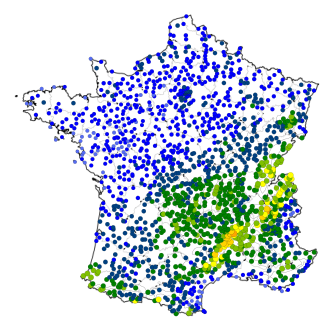
\includegraphics[width=7.9cm]{../outputs/maps/stats_mean-max/quotidien/compare_4/sat_99.5/jja/obs_norast.pdf} & \centering \includegraphics[width=1cm]{../outputs/maps/stats_mean-max/quotidien/compare_4/sat_99.5/legend.pdf} \tabularnewline
\end{longtable*}

\subsection{Données horaires
(1990-2022)}\label{donnuxe9es-horaires-1990-2022-1}

\subsubsection{Par année
hydrologique}\label{par-annuxe9e-hydrologique-1}

\begin{longtable*}{m{2.0cm}m{7.9cm}m{7.9cm}m{1cm}}
 & \centering  & \centering  & \tabularnewline
\centering \textbf{HYDRO} \\[0.2em] \begin{tabular}{r@{\hspace{0.2em}}l}$r$  & $= 0.89$ \\ ME   & $= -3.42$ \\ $n$  & $= 574$ \\ \end{tabular} & \centering 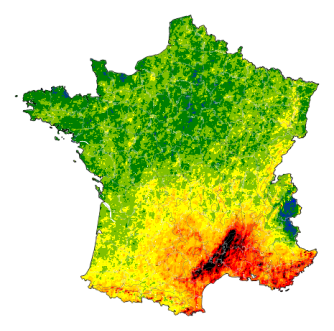
\includegraphics[width=7.9cm]{../outputs/maps/stats_mean-max/horaire/compare_1/sat_99.5/hydro/mod_norast.pdf} & \centering 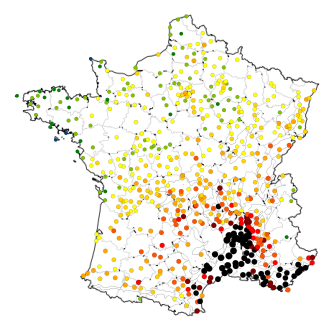
\includegraphics[width=7.9cm]{../outputs/maps/stats_mean-max/horaire/compare_1/sat_99.5/hydro/obs_norast.pdf} & \centering \includegraphics[width=1cm]{../outputs/maps/stats_mean-max/horaire/compare_1/sat_99.5/legend.pdf} \tabularnewline
\end{longtable*}

\subsubsection{Par saison}\label{par-saison-1}

\begin{longtable*}{m{2.0cm}m{7.9cm}m{7.9cm}m{1cm}}
 & \centering  & \centering  & \tabularnewline
\centering \textbf{SON} \\[0.2em] \begin{tabular}{r@{\hspace{0.2em}}l}$r$  & $= 0.93$ \\ ME   & $= -1.18$ \\ $n$  & $= 609$ \\ \end{tabular} & \centering 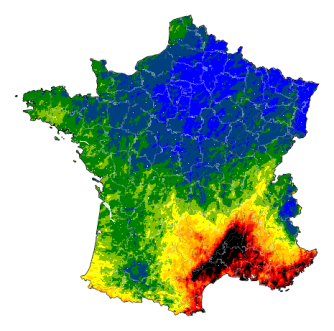
\includegraphics[width=7.9cm]{../outputs/maps/stats_mean-max/horaire/compare_4/sat_99.5/son/mod_norast.pdf} & \centering 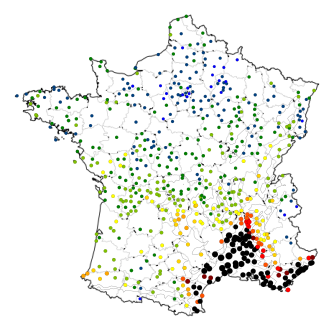
\includegraphics[width=7.9cm]{../outputs/maps/stats_mean-max/horaire/compare_4/sat_99.5/son/obs_norast.pdf} & \centering \includegraphics[width=1cm]{../outputs/maps/stats_mean-max/horaire/compare_4/sat_99.5/legend.pdf} \tabularnewline
\centering \textbf{DJF} \\[0.2em] \begin{tabular}{r@{\hspace{0.2em}}l}$r$  & $= 0.91$ \\ ME   & $= -0.02$ \\ $n$  & $= 511$ \\ \end{tabular} & \centering 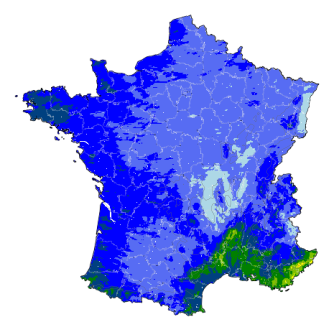
\includegraphics[width=7.9cm]{../outputs/maps/stats_mean-max/horaire/compare_4/sat_99.5/djf/mod_norast.pdf} & \centering 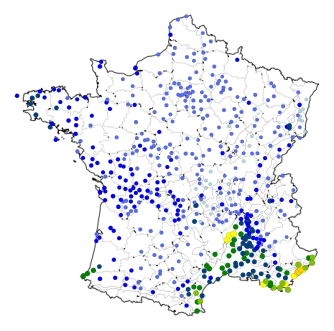
\includegraphics[width=7.9cm]{../outputs/maps/stats_mean-max/horaire/compare_4/sat_99.5/djf/obs_norast.pdf} & \centering \includegraphics[width=1cm]{../outputs/maps/stats_mean-max/horaire/compare_4/sat_99.5/legend.pdf} \tabularnewline
\centering \textbf{MAM} \\[0.2em] \begin{tabular}{r@{\hspace{0.2em}}l}$r$  & $= 0.70$ \\ ME   & $= -0.13$ \\ $n$  & $= 589$ \\ \end{tabular} & \centering 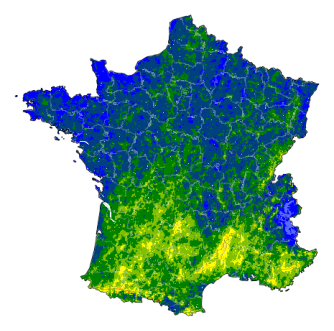
\includegraphics[width=7.9cm]{../outputs/maps/stats_mean-max/horaire/compare_4/sat_99.5/mam/mod_norast.pdf} & \centering 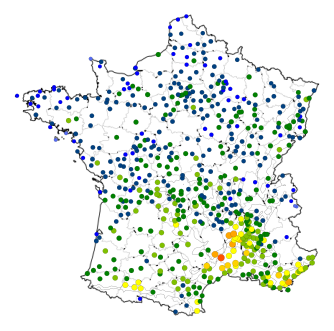
\includegraphics[width=7.9cm]{../outputs/maps/stats_mean-max/horaire/compare_4/sat_99.5/mam/obs_norast.pdf} & \centering \includegraphics[width=1cm]{../outputs/maps/stats_mean-max/horaire/compare_4/sat_99.5/legend.pdf} \tabularnewline
\centering \textbf{JJA} \\[0.2em] \begin{tabular}{r@{\hspace{0.2em}}l}$r$  & $= 0.70$ \\ ME   & $= -3.75$ \\ $n$  & $= 606$ \\ \end{tabular} & \centering 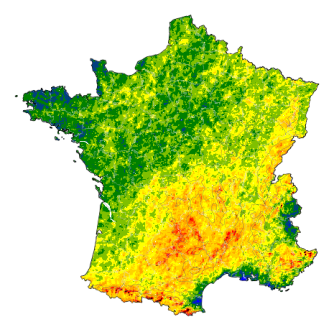
\includegraphics[width=7.9cm]{../outputs/maps/stats_mean-max/horaire/compare_4/sat_99.5/jja/mod_norast.pdf} & \centering 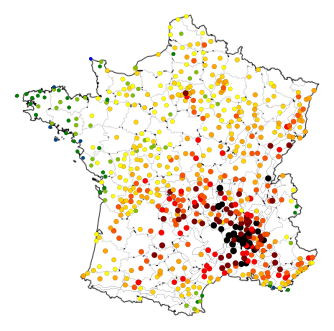
\includegraphics[width=7.9cm]{../outputs/maps/stats_mean-max/horaire/compare_4/sat_99.5/jja/obs_norast.pdf} & \centering \includegraphics[width=1cm]{../outputs/maps/stats_mean-max/horaire/compare_4/sat_99.5/legend.pdf} \tabularnewline
\end{longtable*}

\section{Tendances relatives du niveau de retour 10 ans estimée par le
meilleur
modèle}\label{tendances-relatives-du-niveau-de-retour-10-ans-estimuxe9e-par-le-meilleur-moduxe8le}

Saturation des 1\% valeurs les plus extrêmes.

\subsection{Données journalières
(1959-2022)}\label{donnuxe9es-journaliuxe8res-1959-2022-2}

\subsubsection{Par année
hydrologique}\label{par-annuxe9e-hydrologique-2}

\begin{longtable*}{m{2.0cm}m{7.9cm}m{7.9cm}m{1cm}}
 & \centering  & \centering  & \tabularnewline
\centering \textbf{SON} \\[0.2em] \begin{tabular}{r@{\hspace{0.2em}}l}$r$  & $= 0.21$ \\ ME   & $= -1.44$ \\ $n$  & $= 1664$ \\ \end{tabular} & \centering \includegraphics[width=7.9cm]{../outputs/maps/gev_z_T_p/quotidien/compare_4/sat_99.0/son/mod_norast.pdf} & \centering \includegraphics[width=7.9cm]{../outputs/maps/gev_z_T_p/quotidien/compare_4/sat_99.0/son/obs_norast.pdf} & \centering \includegraphics[width=1cm]{../outputs/maps/gev_z_T_p/quotidien/compare_4/sat_99.0/legend.pdf} \tabularnewline
\centering \textbf{DJF} \\[0.2em] \begin{tabular}{r@{\hspace{0.2em}}l}$r$  & $= 0.23$ \\ ME   & $= -1.89$ \\ $n$  & $= 1603$ \\ \end{tabular} & \centering \includegraphics[width=7.9cm]{../outputs/maps/gev_z_T_p/quotidien/compare_4/sat_99.0/djf/mod_norast.pdf} & \centering \includegraphics[width=7.9cm]{../outputs/maps/gev_z_T_p/quotidien/compare_4/sat_99.0/djf/obs_norast.pdf} & \centering \includegraphics[width=1cm]{../outputs/maps/gev_z_T_p/quotidien/compare_4/sat_99.0/legend.pdf} \tabularnewline
\centering \textbf{MAM} \\[0.2em] \begin{tabular}{r@{\hspace{0.2em}}l}$r$  & $= 0.21$ \\ ME   & $= -1.00$ \\ $n$  & $= 1650$ \\ \end{tabular} & \centering \includegraphics[width=7.9cm]{../outputs/maps/gev_z_T_p/quotidien/compare_4/sat_99.0/mam/mod_norast.pdf} & \centering \includegraphics[width=7.9cm]{../outputs/maps/gev_z_T_p/quotidien/compare_4/sat_99.0/mam/obs_norast.pdf} & \centering \includegraphics[width=1cm]{../outputs/maps/gev_z_T_p/quotidien/compare_4/sat_99.0/legend.pdf} \tabularnewline
\centering \textbf{JJA} \\[0.2em] \begin{tabular}{r@{\hspace{0.2em}}l}$r$  & $= 0.16$ \\ ME   & $= -3.79$ \\ $n$  & $= 1640$ \\ \end{tabular} & \centering \includegraphics[width=7.9cm]{../outputs/maps/gev_z_T_p/quotidien/compare_4/sat_99.0/jja/mod_norast.pdf} & \centering \includegraphics[width=7.9cm]{../outputs/maps/gev_z_T_p/quotidien/compare_4/sat_99.0/jja/obs_norast.pdf} & \centering \includegraphics[width=1cm]{../outputs/maps/gev_z_T_p/quotidien/compare_4/sat_99.0/legend.pdf} \tabularnewline
\end{longtable*}

\subsubsection{Par saison}\label{par-saison-2}

\begin{longtable*}{m{2.0cm}m{7.9cm}m{7.9cm}m{1cm}}
 & \centering  & \centering  & \tabularnewline
\centering \textbf{JAN} \\[0.2em] \begin{tabular}{r@{\hspace{0.2em}}l}$r$  & $= 0.41$ \\ ME   & $= -2.75$ \\ $n$  & $= 1672$ \\ \end{tabular} & \centering \includegraphics[width=7.9cm]{../outputs/maps/gev_z_T_p/quotidien/compare_12/sat_99.0/jan/mod_norast.pdf} & \centering \includegraphics[width=7.9cm]{../outputs/maps/gev_z_T_p/quotidien/compare_12/sat_99.0/jan/obs_norast.pdf} & \centering \includegraphics[width=1cm]{../outputs/maps/gev_z_T_p/quotidien/compare_12/sat_99.0/legend.pdf} \tabularnewline
\centering \textbf{FEV} \\[0.2em] \begin{tabular}{r@{\hspace{0.2em}}l}$r$  & $= 0.33$ \\ ME   & $= -0.57$ \\ $n$  & $= 1677$ \\ \end{tabular} & \centering \includegraphics[width=7.9cm]{../outputs/maps/gev_z_T_p/quotidien/compare_12/sat_99.0/fev/mod_norast.pdf} & \centering \includegraphics[width=7.9cm]{../outputs/maps/gev_z_T_p/quotidien/compare_12/sat_99.0/fev/obs_norast.pdf} & \centering \includegraphics[width=1cm]{../outputs/maps/gev_z_T_p/quotidien/compare_12/sat_99.0/legend.pdf} \tabularnewline
\centering \textbf{MAR} \\[0.2em] \begin{tabular}{r@{\hspace{0.2em}}l}$r$  & $= 0.42$ \\ ME   & $= -0.36$ \\ $n$  & $= 1678$ \\ \end{tabular} & \centering \includegraphics[width=7.9cm]{../outputs/maps/gev_z_T_p/quotidien/compare_12/sat_99.0/mar/mod_norast.pdf} & \centering \includegraphics[width=7.9cm]{../outputs/maps/gev_z_T_p/quotidien/compare_12/sat_99.0/mar/obs_norast.pdf} & \centering \includegraphics[width=1cm]{../outputs/maps/gev_z_T_p/quotidien/compare_12/sat_99.0/legend.pdf} \tabularnewline
\centering \textbf{AVR} \\[0.2em] \begin{tabular}{r@{\hspace{0.2em}}l}$r$  & $= 0.19$ \\ ME   & $= -3.12$ \\ $n$  & $= 1681$ \\ \end{tabular} & \centering \includegraphics[width=7.9cm]{../outputs/maps/gev_z_T_p/quotidien/compare_12/sat_99.0/avr/mod_norast.pdf} & \centering \includegraphics[width=7.9cm]{../outputs/maps/gev_z_T_p/quotidien/compare_12/sat_99.0/avr/obs_norast.pdf} & \centering \includegraphics[width=1cm]{../outputs/maps/gev_z_T_p/quotidien/compare_12/sat_99.0/legend.pdf} \tabularnewline
\centering \textbf{MAI} \\[0.2em] \begin{tabular}{r@{\hspace{0.2em}}l}$r$  & $= 0.27$ \\ ME   & $= -0.86$ \\ $n$  & $= 1682$ \\ \end{tabular} & \centering \includegraphics[width=7.9cm]{../outputs/maps/gev_z_T_p/quotidien/compare_12/sat_99.0/mai/mod_norast.pdf} & \centering \includegraphics[width=7.9cm]{../outputs/maps/gev_z_T_p/quotidien/compare_12/sat_99.0/mai/obs_norast.pdf} & \centering \includegraphics[width=1cm]{../outputs/maps/gev_z_T_p/quotidien/compare_12/sat_99.0/legend.pdf} \tabularnewline
\centering \textbf{JUI} \\[0.2em] \begin{tabular}{r@{\hspace{0.2em}}l}$r$  & $= 0.07$ \\ ME   & $= -2.27$ \\ $n$  & $= 1685$ \\ \end{tabular} & \centering \includegraphics[width=7.9cm]{../outputs/maps/gev_z_T_p/quotidien/compare_12/sat_99.0/jui/mod_norast.pdf} & \centering \includegraphics[width=7.9cm]{../outputs/maps/gev_z_T_p/quotidien/compare_12/sat_99.0/jui/obs_norast.pdf} & \centering \includegraphics[width=1cm]{../outputs/maps/gev_z_T_p/quotidien/compare_12/sat_99.0/legend.pdf} \tabularnewline
\centering \textbf{JUILL} \\[0.2em] \begin{tabular}{r@{\hspace{0.2em}}l}$r$  & $= 0.25$ \\ ME   & $= -1.94$ \\ $n$  & $= 1682$ \\ \end{tabular} & \centering \includegraphics[width=7.9cm]{../outputs/maps/gev_z_T_p/quotidien/compare_12/sat_99.0/juill/mod_norast.pdf} & \centering \includegraphics[width=7.9cm]{../outputs/maps/gev_z_T_p/quotidien/compare_12/sat_99.0/juill/obs_norast.pdf} & \centering \includegraphics[width=1cm]{../outputs/maps/gev_z_T_p/quotidien/compare_12/sat_99.0/legend.pdf} \tabularnewline
\centering \textbf{AOU} \\[0.2em] \begin{tabular}{r@{\hspace{0.2em}}l}$r$  & $= 0.40$ \\ ME   & $= -8.14$ \\ $n$  & $= 1685$ \\ \end{tabular} & \centering \includegraphics[width=7.9cm]{../outputs/maps/gev_z_T_p/quotidien/compare_12/sat_99.0/aou/mod_norast.pdf} & \centering \includegraphics[width=7.9cm]{../outputs/maps/gev_z_T_p/quotidien/compare_12/sat_99.0/aou/obs_norast.pdf} & \centering \includegraphics[width=1cm]{../outputs/maps/gev_z_T_p/quotidien/compare_12/sat_99.0/legend.pdf} \tabularnewline
\centering \textbf{SEP} \\[0.2em] \begin{tabular}{r@{\hspace{0.2em}}l}$r$  & $= 0.27$ \\ ME   & $= -4.55$ \\ $n$  & $= 1690$ \\ \end{tabular} & \centering \includegraphics[width=7.9cm]{../outputs/maps/gev_z_T_p/quotidien/compare_12/sat_99.0/sep/mod_norast.pdf} & \centering \includegraphics[width=7.9cm]{../outputs/maps/gev_z_T_p/quotidien/compare_12/sat_99.0/sep/obs_norast.pdf} & \centering \includegraphics[width=1cm]{../outputs/maps/gev_z_T_p/quotidien/compare_12/sat_99.0/legend.pdf} \tabularnewline
\centering \textbf{OCT} \\[0.2em] \begin{tabular}{r@{\hspace{0.2em}}l}$r$  & $= 0.23$ \\ ME   & $= 0.55$ \\ $n$  & $= 1693$ \\ \end{tabular} & \centering \includegraphics[width=7.9cm]{../outputs/maps/gev_z_T_p/quotidien/compare_12/sat_99.0/oct/mod_norast.pdf} & \centering \includegraphics[width=7.9cm]{../outputs/maps/gev_z_T_p/quotidien/compare_12/sat_99.0/oct/obs_norast.pdf} & \centering \includegraphics[width=1cm]{../outputs/maps/gev_z_T_p/quotidien/compare_12/sat_99.0/legend.pdf} \tabularnewline
\centering \textbf{NOV} \\[0.2em] \begin{tabular}{r@{\hspace{0.2em}}l}$r$  & $= 0.48$ \\ ME   & $= -0.68$ \\ $n$  & $= 1705$ \\ \end{tabular} & \centering \includegraphics[width=7.9cm]{../outputs/maps/gev_z_T_p/quotidien/compare_12/sat_99.0/nov/mod_norast.pdf} & \centering \includegraphics[width=7.9cm]{../outputs/maps/gev_z_T_p/quotidien/compare_12/sat_99.0/nov/obs_norast.pdf} & \centering \includegraphics[width=1cm]{../outputs/maps/gev_z_T_p/quotidien/compare_12/sat_99.0/legend.pdf} \tabularnewline
\centering \textbf{DEC} \\[0.2em] \begin{tabular}{r@{\hspace{0.2em}}l}$r$  & $= 0.51$ \\ ME   & $= -0.02$ \\ $n$  & $= 1692$ \\ \end{tabular} & \centering \includegraphics[width=7.9cm]{../outputs/maps/gev_z_T_p/quotidien/compare_12/sat_99.0/dec/mod_norast.pdf} & \centering \includegraphics[width=7.9cm]{../outputs/maps/gev_z_T_p/quotidien/compare_12/sat_99.0/dec/obs_norast.pdf} & \centering \includegraphics[width=1cm]{../outputs/maps/gev_z_T_p/quotidien/compare_12/sat_99.0/legend.pdf} \tabularnewline
\end{longtable*}

\subsection{Données journalières
(1990-2022)}\label{donnuxe9es-journaliuxe8res-1990-2022}

\subsubsection{Par année
hydrologique}\label{par-annuxe9e-hydrologique-3}

\begin{longtable*}{m{2.0cm}m{7.9cm}m{7.9cm}m{1cm}}
 & \centering  & \centering  & \tabularnewline
\centering \textbf{SON} \\[0.2em] \begin{tabular}{r@{\hspace{0.2em}}l}$r$  & $= 0.13$ \\ ME   & $= -1.93$ \\ $n$  & $= 2719$ \\ \end{tabular} & \centering \includegraphics[width=7.9cm]{../outputs/maps/gev_z_T_p/quotidien_reduce/compare_4/sat_99.0/son/mod_norast.pdf} & \centering \includegraphics[width=7.9cm]{../outputs/maps/gev_z_T_p/quotidien_reduce/compare_4/sat_99.0/son/obs_norast.pdf} & \centering \includegraphics[width=1cm]{../outputs/maps/gev_z_T_p/quotidien_reduce/compare_4/sat_99.0/legend.pdf} \tabularnewline
\centering \textbf{DJF} \\[0.2em] \begin{tabular}{r@{\hspace{0.2em}}l}$r$  & $= 0.29$ \\ ME   & $= -0.09$ \\ $n$  & $= 2663$ \\ \end{tabular} & \centering \includegraphics[width=7.9cm]{../outputs/maps/gev_z_T_p/quotidien_reduce/compare_4/sat_99.0/djf/mod_norast.pdf} & \centering \includegraphics[width=7.9cm]{../outputs/maps/gev_z_T_p/quotidien_reduce/compare_4/sat_99.0/djf/obs_norast.pdf} & \centering \includegraphics[width=1cm]{../outputs/maps/gev_z_T_p/quotidien_reduce/compare_4/sat_99.0/legend.pdf} \tabularnewline
\centering \textbf{MAM} \\[0.2em] \begin{tabular}{r@{\hspace{0.2em}}l}$r$  & $= 0.21$ \\ ME   & $= -1.47$ \\ $n$  & $= 2729$ \\ \end{tabular} & \centering \includegraphics[width=7.9cm]{../outputs/maps/gev_z_T_p/quotidien_reduce/compare_4/sat_99.0/mam/mod_norast.pdf} & \centering \includegraphics[width=7.9cm]{../outputs/maps/gev_z_T_p/quotidien_reduce/compare_4/sat_99.0/mam/obs_norast.pdf} & \centering \includegraphics[width=1cm]{../outputs/maps/gev_z_T_p/quotidien_reduce/compare_4/sat_99.0/legend.pdf} \tabularnewline
\centering \textbf{JJA} \\[0.2em] \begin{tabular}{r@{\hspace{0.2em}}l}$r$  & $= 0.16$ \\ ME   & $= 0.23$ \\ $n$  & $= 2718$ \\ \end{tabular} & \centering \includegraphics[width=7.9cm]{../outputs/maps/gev_z_T_p/quotidien_reduce/compare_4/sat_99.0/jja/mod_norast.pdf} & \centering \includegraphics[width=7.9cm]{../outputs/maps/gev_z_T_p/quotidien_reduce/compare_4/sat_99.0/jja/obs_norast.pdf} & \centering \includegraphics[width=1cm]{../outputs/maps/gev_z_T_p/quotidien_reduce/compare_4/sat_99.0/legend.pdf} \tabularnewline
\end{longtable*}

\subsubsection{Par saison}\label{par-saison-3}

\begin{longtable*}{m{2.0cm}m{7.9cm}m{7.9cm}m{1cm}}
 & \centering  & \centering  & \tabularnewline
\centering \textbf{JAN} \\[0.2em] \begin{tabular}{r@{\hspace{0.2em}}l}\end{tabular} & \centering \includegraphics[width=7.9cm]{../outputs/maps/gev_z_T_p/quotidien_reduce/compare_12/sat_99.0/jan/mod_norast.pdf} & \centering \includegraphics[width=7.9cm]{../outputs/maps/gev_z_T_p/quotidien_reduce/compare_12/sat_99.0/jan/obs_norast.pdf} & \centering \includegraphics[width=1cm]{../outputs/maps/gev_z_T_p/quotidien_reduce/compare_12/sat_99.0/legend.pdf} \tabularnewline
\centering \textbf{FEV} \\[0.2em] \begin{tabular}{r@{\hspace{0.2em}}l}\end{tabular} & \centering \includegraphics[width=7.9cm]{../outputs/maps/gev_z_T_p/quotidien_reduce/compare_12/sat_99.0/fev/mod_norast.pdf} & \centering \includegraphics[width=7.9cm]{../outputs/maps/gev_z_T_p/quotidien_reduce/compare_12/sat_99.0/fev/obs_norast.pdf} & \centering \includegraphics[width=1cm]{../outputs/maps/gev_z_T_p/quotidien_reduce/compare_12/sat_99.0/legend.pdf} \tabularnewline
\centering \textbf{MAR} \\[0.2em] \begin{tabular}{r@{\hspace{0.2em}}l}\end{tabular} & \centering \includegraphics[width=7.9cm]{../outputs/maps/gev_z_T_p/quotidien_reduce/compare_12/sat_99.0/mar/mod_norast.pdf} & \centering \includegraphics[width=7.9cm]{../outputs/maps/gev_z_T_p/quotidien_reduce/compare_12/sat_99.0/mar/obs_norast.pdf} & \centering \includegraphics[width=1cm]{../outputs/maps/gev_z_T_p/quotidien_reduce/compare_12/sat_99.0/legend.pdf} \tabularnewline
\centering \textbf{AVR} \\[0.2em] \begin{tabular}{r@{\hspace{0.2em}}l}\end{tabular} & \centering \includegraphics[width=7.9cm]{../outputs/maps/gev_z_T_p/quotidien_reduce/compare_12/sat_99.0/avr/mod_norast.pdf} & \centering \includegraphics[width=7.9cm]{../outputs/maps/gev_z_T_p/quotidien_reduce/compare_12/sat_99.0/avr/obs_norast.pdf} & \centering \includegraphics[width=1cm]{../outputs/maps/gev_z_T_p/quotidien_reduce/compare_12/sat_99.0/legend.pdf} \tabularnewline
\centering \textbf{MAI} \\[0.2em] \begin{tabular}{r@{\hspace{0.2em}}l}\end{tabular} & \centering \includegraphics[width=7.9cm]{../outputs/maps/gev_z_T_p/quotidien_reduce/compare_12/sat_99.0/mai/mod_norast.pdf} & \centering \includegraphics[width=7.9cm]{../outputs/maps/gev_z_T_p/quotidien_reduce/compare_12/sat_99.0/mai/obs_norast.pdf} & \centering \includegraphics[width=1cm]{../outputs/maps/gev_z_T_p/quotidien_reduce/compare_12/sat_99.0/legend.pdf} \tabularnewline
\centering \textbf{JUI} \\[0.2em] \begin{tabular}{r@{\hspace{0.2em}}l}\end{tabular} & \centering \includegraphics[width=7.9cm]{../outputs/maps/gev_z_T_p/quotidien_reduce/compare_12/sat_99.0/jui/mod_norast.pdf} & \centering \includegraphics[width=7.9cm]{../outputs/maps/gev_z_T_p/quotidien_reduce/compare_12/sat_99.0/jui/obs_norast.pdf} & \centering \includegraphics[width=1cm]{../outputs/maps/gev_z_T_p/quotidien_reduce/compare_12/sat_99.0/legend.pdf} \tabularnewline
\centering \textbf{JUILL} \\[0.2em] \begin{tabular}{r@{\hspace{0.2em}}l}\end{tabular} & \centering \includegraphics[width=7.9cm]{../outputs/maps/gev_z_T_p/quotidien_reduce/compare_12/sat_99.0/juill/mod_norast.pdf} & \centering \includegraphics[width=7.9cm]{../outputs/maps/gev_z_T_p/quotidien_reduce/compare_12/sat_99.0/juill/obs_norast.pdf} & \centering \includegraphics[width=1cm]{../outputs/maps/gev_z_T_p/quotidien_reduce/compare_12/sat_99.0/legend.pdf} \tabularnewline
\centering \textbf{AOU} \\[0.2em] \begin{tabular}{r@{\hspace{0.2em}}l}\end{tabular} & \centering \includegraphics[width=7.9cm]{../outputs/maps/gev_z_T_p/quotidien_reduce/compare_12/sat_99.0/aou/mod_norast.pdf} & \centering \includegraphics[width=7.9cm]{../outputs/maps/gev_z_T_p/quotidien_reduce/compare_12/sat_99.0/aou/obs_norast.pdf} & \centering \includegraphics[width=1cm]{../outputs/maps/gev_z_T_p/quotidien_reduce/compare_12/sat_99.0/legend.pdf} \tabularnewline
\centering \textbf{SEP} \\[0.2em] \begin{tabular}{r@{\hspace{0.2em}}l}\end{tabular} & \centering \includegraphics[width=7.9cm]{../outputs/maps/gev_z_T_p/quotidien_reduce/compare_12/sat_99.0/sep/mod_norast.pdf} & \centering \includegraphics[width=7.9cm]{../outputs/maps/gev_z_T_p/quotidien_reduce/compare_12/sat_99.0/sep/obs_norast.pdf} & \centering \includegraphics[width=1cm]{../outputs/maps/gev_z_T_p/quotidien_reduce/compare_12/sat_99.0/legend.pdf} \tabularnewline
\centering \textbf{OCT} \\[0.2em] \begin{tabular}{r@{\hspace{0.2em}}l}\end{tabular} & \centering \includegraphics[width=7.9cm]{../outputs/maps/gev_z_T_p/quotidien_reduce/compare_12/sat_99.0/oct/mod_norast.pdf} & \centering \includegraphics[width=7.9cm]{../outputs/maps/gev_z_T_p/quotidien_reduce/compare_12/sat_99.0/oct/obs_norast.pdf} & \centering \includegraphics[width=1cm]{../outputs/maps/gev_z_T_p/quotidien_reduce/compare_12/sat_99.0/legend.pdf} \tabularnewline
\centering \textbf{NOV} \\[0.2em] \begin{tabular}{r@{\hspace{0.2em}}l}\end{tabular} & \centering \includegraphics[width=7.9cm]{../outputs/maps/gev_z_T_p/quotidien_reduce/compare_12/sat_99.0/nov/mod_norast.pdf} & \centering \includegraphics[width=7.9cm]{../outputs/maps/gev_z_T_p/quotidien_reduce/compare_12/sat_99.0/nov/obs_norast.pdf} & \centering \includegraphics[width=1cm]{../outputs/maps/gev_z_T_p/quotidien_reduce/compare_12/sat_99.0/legend.pdf} \tabularnewline
\centering \textbf{DEC} \\[0.2em] \begin{tabular}{r@{\hspace{0.2em}}l}\end{tabular} & \centering \includegraphics[width=7.9cm]{../outputs/maps/gev_z_T_p/quotidien_reduce/compare_12/sat_99.0/dec/mod_norast.pdf} & \centering \includegraphics[width=7.9cm]{../outputs/maps/gev_z_T_p/quotidien_reduce/compare_12/sat_99.0/dec/obs_norast.pdf} & \centering \includegraphics[width=1cm]{../outputs/maps/gev_z_T_p/quotidien_reduce/compare_12/sat_99.0/legend.pdf} \tabularnewline
\end{longtable*}

\subsection{Données horaire
(1990-2022)}\label{donnuxe9es-horaire-1990-2022}

\subsubsection{Par année
hydrologique}\label{par-annuxe9e-hydrologique-4}

\begin{longtable*}{m{2.0cm}m{7.9cm}m{7.9cm}m{1cm}}
 & \centering  & \centering  & \tabularnewline
\centering \textbf{SON} \\[0.2em] \begin{tabular}{r@{\hspace{0.2em}}l}$r$  & $= 0.05$ \\ ME   & $= -9.70$ \\ $n$  & $= 609$ \\ \end{tabular} & \centering \includegraphics[width=7.9cm]{../outputs/maps/gev_z_T_p/horaire/compare_4/sat_99.0/son/mod_norast.pdf} & \centering \includegraphics[width=7.9cm]{../outputs/maps/gev_z_T_p/horaire/compare_4/sat_99.0/son/obs_norast.pdf} & \centering \includegraphics[width=1cm]{../outputs/maps/gev_z_T_p/horaire/compare_4/sat_99.0/legend.pdf} \tabularnewline
\centering \textbf{DJF} \\[0.2em] \begin{tabular}{r@{\hspace{0.2em}}l}$r$  & $= 0.05$ \\ ME   & $= 0.44$ \\ $n$  & $= 511$ \\ \end{tabular} & \centering \includegraphics[width=7.9cm]{../outputs/maps/gev_z_T_p/horaire/compare_4/sat_99.0/djf/mod_norast.pdf} & \centering \includegraphics[width=7.9cm]{../outputs/maps/gev_z_T_p/horaire/compare_4/sat_99.0/djf/obs_norast.pdf} & \centering \includegraphics[width=1cm]{../outputs/maps/gev_z_T_p/horaire/compare_4/sat_99.0/legend.pdf} \tabularnewline
\centering \textbf{MAM} \\[0.2em] \begin{tabular}{r@{\hspace{0.2em}}l}$r$  & $= -0.08$ \\ ME   & $= -10.49$ \\ $n$  & $= 589$ \\ \end{tabular} & \centering \includegraphics[width=7.9cm]{../outputs/maps/gev_z_T_p/horaire/compare_4/sat_99.0/mam/mod_norast.pdf} & \centering \includegraphics[width=7.9cm]{../outputs/maps/gev_z_T_p/horaire/compare_4/sat_99.0/mam/obs_norast.pdf} & \centering \includegraphics[width=1cm]{../outputs/maps/gev_z_T_p/horaire/compare_4/sat_99.0/legend.pdf} \tabularnewline
\centering \textbf{JJA} \\[0.2em] \begin{tabular}{r@{\hspace{0.2em}}l}$r$  & $= -0.04$ \\ ME   & $= -11.16$ \\ $n$  & $= 606$ \\ \end{tabular} & \centering \includegraphics[width=7.9cm]{../outputs/maps/gev_z_T_p/horaire/compare_4/sat_99.0/jja/mod_norast.pdf} & \centering \includegraphics[width=7.9cm]{../outputs/maps/gev_z_T_p/horaire/compare_4/sat_99.0/jja/obs_norast.pdf} & \centering \includegraphics[width=1cm]{../outputs/maps/gev_z_T_p/horaire/compare_4/sat_99.0/legend.pdf} \tabularnewline
\end{longtable*}

\subsubsection{Par saison}\label{par-saison-4}

\begin{longtable*}{m{2.0cm}m{7.9cm}m{7.9cm}m{1cm}}
 & \centering  & \centering  & \tabularnewline
\centering \textbf{JAN} \\[0.2em] \begin{tabular}{r@{\hspace{0.2em}}l}$r$  & $= 0.08$ \\ ME   & $= -3.56$ \\ $n$  & $= 488$ \\ \end{tabular} & \centering \includegraphics[width=7.9cm]{../outputs/maps/gev_z_T_p/horaire/compare_12/sat_99.0/jan/mod_norast.pdf} & \centering \includegraphics[width=7.9cm]{../outputs/maps/gev_z_T_p/horaire/compare_12/sat_99.0/jan/obs_norast.pdf} & \centering \includegraphics[width=1cm]{../outputs/maps/gev_z_T_p/horaire/compare_12/sat_99.0/legend.pdf} \tabularnewline
\centering \textbf{FEV} \\[0.2em] \begin{tabular}{r@{\hspace{0.2em}}l}$r$  & $= 0.42$ \\ ME   & $= -17.21$ \\ $n$  & $= 508$ \\ \end{tabular} & \centering \includegraphics[width=7.9cm]{../outputs/maps/gev_z_T_p/horaire/compare_12/sat_99.0/fev/mod_norast.pdf} & \centering \includegraphics[width=7.9cm]{../outputs/maps/gev_z_T_p/horaire/compare_12/sat_99.0/fev/obs_norast.pdf} & \centering \includegraphics[width=1cm]{../outputs/maps/gev_z_T_p/horaire/compare_12/sat_99.0/legend.pdf} \tabularnewline
\centering \textbf{MAR} \\[0.2em] \begin{tabular}{r@{\hspace{0.2em}}l}$r$  & $= 0.23$ \\ ME   & $= -15.20$ \\ $n$  & $= 588$ \\ \end{tabular} & \centering \includegraphics[width=7.9cm]{../outputs/maps/gev_z_T_p/horaire/compare_12/sat_99.0/mar/mod_norast.pdf} & \centering \includegraphics[width=7.9cm]{../outputs/maps/gev_z_T_p/horaire/compare_12/sat_99.0/mar/obs_norast.pdf} & \centering \includegraphics[width=1cm]{../outputs/maps/gev_z_T_p/horaire/compare_12/sat_99.0/legend.pdf} \tabularnewline
\centering \textbf{AVR} \\[0.2em] \begin{tabular}{r@{\hspace{0.2em}}l}$r$  & $= 0.12$ \\ ME   & $= 0.42$ \\ $n$  & $= 600$ \\ \end{tabular} & \centering \includegraphics[width=7.9cm]{../outputs/maps/gev_z_T_p/horaire/compare_12/sat_99.0/avr/mod_norast.pdf} & \centering \includegraphics[width=7.9cm]{../outputs/maps/gev_z_T_p/horaire/compare_12/sat_99.0/avr/obs_norast.pdf} & \centering \includegraphics[width=1cm]{../outputs/maps/gev_z_T_p/horaire/compare_12/sat_99.0/legend.pdf} \tabularnewline
\centering \textbf{MAI} \\[0.2em] \begin{tabular}{r@{\hspace{0.2em}}l}$r$  & $= 0.07$ \\ ME   & $= -16.32$ \\ $n$  & $= 590$ \\ \end{tabular} & \centering \includegraphics[width=7.9cm]{../outputs/maps/gev_z_T_p/horaire/compare_12/sat_99.0/mai/mod_norast.pdf} & \centering \includegraphics[width=7.9cm]{../outputs/maps/gev_z_T_p/horaire/compare_12/sat_99.0/mai/obs_norast.pdf} & \centering \includegraphics[width=1cm]{../outputs/maps/gev_z_T_p/horaire/compare_12/sat_99.0/legend.pdf} \tabularnewline
\centering \textbf{JUI} \\[0.2em] \begin{tabular}{r@{\hspace{0.2em}}l}$r$  & $= 0.09$ \\ ME   & $= -48.20$ \\ $n$  & $= 600$ \\ \end{tabular} & \centering \includegraphics[width=7.9cm]{../outputs/maps/gev_z_T_p/horaire/compare_12/sat_99.0/jui/mod_norast.pdf} & \centering \includegraphics[width=7.9cm]{../outputs/maps/gev_z_T_p/horaire/compare_12/sat_99.0/jui/obs_norast.pdf} & \centering \includegraphics[width=1cm]{../outputs/maps/gev_z_T_p/horaire/compare_12/sat_99.0/legend.pdf} \tabularnewline
\centering \textbf{JUILL} \\[0.2em] \begin{tabular}{r@{\hspace{0.2em}}l}$r$  & $= 0.03$ \\ ME   & $= 1.41$ \\ $n$  & $= 606$ \\ \end{tabular} & \centering \includegraphics[width=7.9cm]{../outputs/maps/gev_z_T_p/horaire/compare_12/sat_99.0/juill/mod_norast.pdf} & \centering \includegraphics[width=7.9cm]{../outputs/maps/gev_z_T_p/horaire/compare_12/sat_99.0/juill/obs_norast.pdf} & \centering \includegraphics[width=1cm]{../outputs/maps/gev_z_T_p/horaire/compare_12/sat_99.0/legend.pdf} \tabularnewline
\centering \textbf{AOU} \\[0.2em] \begin{tabular}{r@{\hspace{0.2em}}l}$r$  & $= 0.09$ \\ ME   & $= -12.48$ \\ $n$  & $= 602$ \\ \end{tabular} & \centering \includegraphics[width=7.9cm]{../outputs/maps/gev_z_T_p/horaire/compare_12/sat_99.0/aou/mod_norast.pdf} & \centering \includegraphics[width=7.9cm]{../outputs/maps/gev_z_T_p/horaire/compare_12/sat_99.0/aou/obs_norast.pdf} & \centering \includegraphics[width=1cm]{../outputs/maps/gev_z_T_p/horaire/compare_12/sat_99.0/legend.pdf} \tabularnewline
\centering \textbf{SEP} \\[0.2em] \begin{tabular}{r@{\hspace{0.2em}}l}$r$  & $= 0.02$ \\ ME   & $= -14.77$ \\ $n$  & $= 620$ \\ \end{tabular} & \centering \includegraphics[width=7.9cm]{../outputs/maps/gev_z_T_p/horaire/compare_12/sat_99.0/sep/mod_norast.pdf} & \centering \includegraphics[width=7.9cm]{../outputs/maps/gev_z_T_p/horaire/compare_12/sat_99.0/sep/obs_norast.pdf} & \centering \includegraphics[width=1cm]{../outputs/maps/gev_z_T_p/horaire/compare_12/sat_99.0/legend.pdf} \tabularnewline
\centering \textbf{OCT} \\[0.2em] \begin{tabular}{r@{\hspace{0.2em}}l}$r$  & $= 0.02$ \\ ME   & $= -9.91$ \\ $n$  & $= 606$ \\ \end{tabular} & \centering \includegraphics[width=7.9cm]{../outputs/maps/gev_z_T_p/horaire/compare_12/sat_99.0/oct/mod_norast.pdf} & \centering \includegraphics[width=7.9cm]{../outputs/maps/gev_z_T_p/horaire/compare_12/sat_99.0/oct/obs_norast.pdf} & \centering \includegraphics[width=1cm]{../outputs/maps/gev_z_T_p/horaire/compare_12/sat_99.0/legend.pdf} \tabularnewline
\centering \textbf{NOV} \\[0.2em] \begin{tabular}{r@{\hspace{0.2em}}l}$r$  & $= 0.16$ \\ ME   & $= 8.69$ \\ $n$  & $= 593$ \\ \end{tabular} & \centering \includegraphics[width=7.9cm]{../outputs/maps/gev_z_T_p/horaire/compare_12/sat_99.0/nov/mod_norast.pdf} & \centering \includegraphics[width=7.9cm]{../outputs/maps/gev_z_T_p/horaire/compare_12/sat_99.0/nov/obs_norast.pdf} & \centering \includegraphics[width=1cm]{../outputs/maps/gev_z_T_p/horaire/compare_12/sat_99.0/legend.pdf} \tabularnewline
\centering \textbf{DEC} \\[0.2em] \begin{tabular}{r@{\hspace{0.2em}}l}$r$  & $= 0.17$ \\ ME   & $= -5.44$ \\ $n$  & $= 548$ \\ \end{tabular} & \centering \includegraphics[width=7.9cm]{../outputs/maps/gev_z_T_p/horaire/compare_12/sat_99.0/dec/mod_norast.pdf} & \centering \includegraphics[width=7.9cm]{../outputs/maps/gev_z_T_p/horaire/compare_12/sat_99.0/dec/obs_norast.pdf} & \centering \includegraphics[width=1cm]{../outputs/maps/gev_z_T_p/horaire/compare_12/sat_99.0/legend.pdf} \tabularnewline
\end{longtable*}

\section{Significativité de la
tendance}\label{significativituxe9-de-la-tendance}

\subsection{Données journalières
(1959-2022)}\label{donnuxe9es-journaliuxe8res-1959-2022-3}

\subsubsection{Par année
hydrologique}\label{par-annuxe9e-hydrologique-5}

\begin{longtable*}{m{2.0cm}m{7.9cm}m{7.9cm}m{1cm}}
 & \centering  & \centering  & \tabularnewline
\centering \textbf{SON} \\[0.2em] \begin{tabular}{r@{\hspace{0.2em}}l}\end{tabular} & \centering \includegraphics[width=7.9cm]{../outputs/maps/gev_significant/quotidien/compare_4/sat_100.0/son/mod_norast.pdf} & \centering \includegraphics[width=7.9cm]{../outputs/maps/gev_significant/quotidien/compare_4/sat_100.0/son/obs_norast.pdf} & \centering \includegraphics[width=1cm]{../outputs/maps/gev_significant/quotidien/compare_4/sat_100.0/legend.pdf} \tabularnewline
\centering \textbf{DJF} \\[0.2em] \begin{tabular}{r@{\hspace{0.2em}}l}\end{tabular} & \centering \includegraphics[width=7.9cm]{../outputs/maps/gev_significant/quotidien/compare_4/sat_100.0/djf/mod_norast.pdf} & \centering \includegraphics[width=7.9cm]{../outputs/maps/gev_significant/quotidien/compare_4/sat_100.0/djf/obs_norast.pdf} & \centering \includegraphics[width=1cm]{../outputs/maps/gev_significant/quotidien/compare_4/sat_100.0/legend.pdf} \tabularnewline
\centering \textbf{MAM} \\[0.2em] \begin{tabular}{r@{\hspace{0.2em}}l}\end{tabular} & \centering \includegraphics[width=7.9cm]{../outputs/maps/gev_significant/quotidien/compare_4/sat_100.0/mam/mod_norast.pdf} & \centering \includegraphics[width=7.9cm]{../outputs/maps/gev_significant/quotidien/compare_4/sat_100.0/mam/obs_norast.pdf} & \centering \includegraphics[width=1cm]{../outputs/maps/gev_significant/quotidien/compare_4/sat_100.0/legend.pdf} \tabularnewline
\centering \textbf{JJA} \\[0.2em] \begin{tabular}{r@{\hspace{0.2em}}l}\end{tabular} & \centering \includegraphics[width=7.9cm]{../outputs/maps/gev_significant/quotidien/compare_4/sat_100.0/jja/mod_norast.pdf} & \centering \includegraphics[width=7.9cm]{../outputs/maps/gev_significant/quotidien/compare_4/sat_100.0/jja/obs_norast.pdf} & \centering \includegraphics[width=1cm]{../outputs/maps/gev_significant/quotidien/compare_4/sat_100.0/legend.pdf} \tabularnewline
\end{longtable*}

\subsubsection{Par saison}\label{par-saison-5}

\begin{longtable*}{m{2.0cm}m{7.9cm}m{7.9cm}m{1cm}}
 & \centering  & \centering  & \tabularnewline
\centering \textbf{JAN} \\[0.2em] \begin{tabular}{r@{\hspace{0.2em}}l}\end{tabular} & \centering \includegraphics[width=7.9cm]{../outputs/maps/gev_significant/quotidien/compare_12/sat_100.0/jan/mod_norast.pdf} & \centering \includegraphics[width=7.9cm]{../outputs/maps/gev_significant/quotidien/compare_12/sat_100.0/jan/obs_norast.pdf} & \centering \includegraphics[width=1cm]{../outputs/maps/gev_significant/quotidien/compare_12/sat_100.0/legend.pdf} \tabularnewline
\centering \textbf{FEV} \\[0.2em] \begin{tabular}{r@{\hspace{0.2em}}l}\end{tabular} & \centering \includegraphics[width=7.9cm]{../outputs/maps/gev_significant/quotidien/compare_12/sat_100.0/fev/mod_norast.pdf} & \centering \includegraphics[width=7.9cm]{../outputs/maps/gev_significant/quotidien/compare_12/sat_100.0/fev/obs_norast.pdf} & \centering \includegraphics[width=1cm]{../outputs/maps/gev_significant/quotidien/compare_12/sat_100.0/legend.pdf} \tabularnewline
\centering \textbf{MAR} \\[0.2em] \begin{tabular}{r@{\hspace{0.2em}}l}\end{tabular} & \centering \includegraphics[width=7.9cm]{../outputs/maps/gev_significant/quotidien/compare_12/sat_100.0/mar/mod_norast.pdf} & \centering \includegraphics[width=7.9cm]{../outputs/maps/gev_significant/quotidien/compare_12/sat_100.0/mar/obs_norast.pdf} & \centering \includegraphics[width=1cm]{../outputs/maps/gev_significant/quotidien/compare_12/sat_100.0/legend.pdf} \tabularnewline
\centering \textbf{AVR} \\[0.2em] \begin{tabular}{r@{\hspace{0.2em}}l}\end{tabular} & \centering \includegraphics[width=7.9cm]{../outputs/maps/gev_significant/quotidien/compare_12/sat_100.0/avr/mod_norast.pdf} & \centering \includegraphics[width=7.9cm]{../outputs/maps/gev_significant/quotidien/compare_12/sat_100.0/avr/obs_norast.pdf} & \centering \includegraphics[width=1cm]{../outputs/maps/gev_significant/quotidien/compare_12/sat_100.0/legend.pdf} \tabularnewline
\centering \textbf{MAI} \\[0.2em] \begin{tabular}{r@{\hspace{0.2em}}l}\end{tabular} & \centering \includegraphics[width=7.9cm]{../outputs/maps/gev_significant/quotidien/compare_12/sat_100.0/mai/mod_norast.pdf} & \centering \includegraphics[width=7.9cm]{../outputs/maps/gev_significant/quotidien/compare_12/sat_100.0/mai/obs_norast.pdf} & \centering \includegraphics[width=1cm]{../outputs/maps/gev_significant/quotidien/compare_12/sat_100.0/legend.pdf} \tabularnewline
\centering \textbf{JUI} \\[0.2em] \begin{tabular}{r@{\hspace{0.2em}}l}\end{tabular} & \centering \includegraphics[width=7.9cm]{../outputs/maps/gev_significant/quotidien/compare_12/sat_100.0/jui/mod_norast.pdf} & \centering \includegraphics[width=7.9cm]{../outputs/maps/gev_significant/quotidien/compare_12/sat_100.0/jui/obs_norast.pdf} & \centering \includegraphics[width=1cm]{../outputs/maps/gev_significant/quotidien/compare_12/sat_100.0/legend.pdf} \tabularnewline
\centering \textbf{JUILL} \\[0.2em] \begin{tabular}{r@{\hspace{0.2em}}l}\end{tabular} & \centering \includegraphics[width=7.9cm]{../outputs/maps/gev_significant/quotidien/compare_12/sat_100.0/juill/mod_norast.pdf} & \centering \includegraphics[width=7.9cm]{../outputs/maps/gev_significant/quotidien/compare_12/sat_100.0/juill/obs_norast.pdf} & \centering \includegraphics[width=1cm]{../outputs/maps/gev_significant/quotidien/compare_12/sat_100.0/legend.pdf} \tabularnewline
\centering \textbf{AOU} \\[0.2em] \begin{tabular}{r@{\hspace{0.2em}}l}\end{tabular} & \centering \includegraphics[width=7.9cm]{../outputs/maps/gev_significant/quotidien/compare_12/sat_100.0/aou/mod_norast.pdf} & \centering \includegraphics[width=7.9cm]{../outputs/maps/gev_significant/quotidien/compare_12/sat_100.0/aou/obs_norast.pdf} & \centering \includegraphics[width=1cm]{../outputs/maps/gev_significant/quotidien/compare_12/sat_100.0/legend.pdf} \tabularnewline
\centering \textbf{SEP} \\[0.2em] \begin{tabular}{r@{\hspace{0.2em}}l}\end{tabular} & \centering \includegraphics[width=7.9cm]{../outputs/maps/gev_significant/quotidien/compare_12/sat_100.0/sep/mod_norast.pdf} & \centering \includegraphics[width=7.9cm]{../outputs/maps/gev_significant/quotidien/compare_12/sat_100.0/sep/obs_norast.pdf} & \centering \includegraphics[width=1cm]{../outputs/maps/gev_significant/quotidien/compare_12/sat_100.0/legend.pdf} \tabularnewline
\centering \textbf{OCT} \\[0.2em] \begin{tabular}{r@{\hspace{0.2em}}l}\end{tabular} & \centering \includegraphics[width=7.9cm]{../outputs/maps/gev_significant/quotidien/compare_12/sat_100.0/oct/mod_norast.pdf} & \centering \includegraphics[width=7.9cm]{../outputs/maps/gev_significant/quotidien/compare_12/sat_100.0/oct/obs_norast.pdf} & \centering \includegraphics[width=1cm]{../outputs/maps/gev_significant/quotidien/compare_12/sat_100.0/legend.pdf} \tabularnewline
\centering \textbf{NOV} \\[0.2em] \begin{tabular}{r@{\hspace{0.2em}}l}\end{tabular} & \centering \includegraphics[width=7.9cm]{../outputs/maps/gev_significant/quotidien/compare_12/sat_100.0/nov/mod_norast.pdf} & \centering \includegraphics[width=7.9cm]{../outputs/maps/gev_significant/quotidien/compare_12/sat_100.0/nov/obs_norast.pdf} & \centering \includegraphics[width=1cm]{../outputs/maps/gev_significant/quotidien/compare_12/sat_100.0/legend.pdf} \tabularnewline
\centering \textbf{DEC} \\[0.2em] \begin{tabular}{r@{\hspace{0.2em}}l}\end{tabular} & \centering \includegraphics[width=7.9cm]{../outputs/maps/gev_significant/quotidien/compare_12/sat_100.0/dec/mod_norast.pdf} & \centering \includegraphics[width=7.9cm]{../outputs/maps/gev_significant/quotidien/compare_12/sat_100.0/dec/obs_norast.pdf} & \centering \includegraphics[width=1cm]{../outputs/maps/gev_significant/quotidien/compare_12/sat_100.0/legend.pdf} \tabularnewline
\end{longtable*}

\subsection{Données journalières
(1990-2022)}\label{donnuxe9es-journaliuxe8res-1990-2022-1}

\subsubsection{Par année
hydrologique}\label{par-annuxe9e-hydrologique-6}

\begin{longtable*}{m{2.0cm}m{7.9cm}m{7.9cm}m{1cm}}
 & \centering  & \centering  & \tabularnewline
\centering \textbf{SON} \\[0.2em] \begin{tabular}{r@{\hspace{0.2em}}l}\end{tabular} & \centering \includegraphics[width=7.9cm]{../outputs/maps/gev_significant/quotidien_reduce/compare_4/sat_100.0/son/mod_norast.pdf} & \centering \includegraphics[width=7.9cm]{../outputs/maps/gev_significant/quotidien_reduce/compare_4/sat_100.0/son/obs_norast.pdf} & \centering \includegraphics[width=1cm]{../outputs/maps/gev_significant/quotidien_reduce/compare_4/sat_100.0/legend.pdf} \tabularnewline
\centering \textbf{DJF} \\[0.2em] \begin{tabular}{r@{\hspace{0.2em}}l}\end{tabular} & \centering \includegraphics[width=7.9cm]{../outputs/maps/gev_significant/quotidien_reduce/compare_4/sat_100.0/djf/mod_norast.pdf} & \centering \includegraphics[width=7.9cm]{../outputs/maps/gev_significant/quotidien_reduce/compare_4/sat_100.0/djf/obs_norast.pdf} & \centering \includegraphics[width=1cm]{../outputs/maps/gev_significant/quotidien_reduce/compare_4/sat_100.0/legend.pdf} \tabularnewline
\centering \textbf{MAM} \\[0.2em] \begin{tabular}{r@{\hspace{0.2em}}l}\end{tabular} & \centering \includegraphics[width=7.9cm]{../outputs/maps/gev_significant/quotidien_reduce/compare_4/sat_100.0/mam/mod_norast.pdf} & \centering \includegraphics[width=7.9cm]{../outputs/maps/gev_significant/quotidien_reduce/compare_4/sat_100.0/mam/obs_norast.pdf} & \centering \includegraphics[width=1cm]{../outputs/maps/gev_significant/quotidien_reduce/compare_4/sat_100.0/legend.pdf} \tabularnewline
\centering \textbf{JJA} \\[0.2em] \begin{tabular}{r@{\hspace{0.2em}}l}\end{tabular} & \centering \includegraphics[width=7.9cm]{../outputs/maps/gev_significant/quotidien_reduce/compare_4/sat_100.0/jja/mod_norast.pdf} & \centering \includegraphics[width=7.9cm]{../outputs/maps/gev_significant/quotidien_reduce/compare_4/sat_100.0/jja/obs_norast.pdf} & \centering \includegraphics[width=1cm]{../outputs/maps/gev_significant/quotidien_reduce/compare_4/sat_100.0/legend.pdf} \tabularnewline
\end{longtable*}

\subsubsection{Par saison}\label{par-saison-6}

\begin{longtable*}{m{2.0cm}m{7.9cm}m{7.9cm}m{1cm}}
 & \centering  & \centering  & \tabularnewline
\centering \textbf{JAN} \\[0.2em] \begin{tabular}{r@{\hspace{0.2em}}l}\end{tabular} & \centering \includegraphics[width=7.9cm]{../outputs/maps/gev_significant/quotidien_reduce/compare_12/sat_100.0/jan/mod_norast.pdf} & \centering \includegraphics[width=7.9cm]{../outputs/maps/gev_significant/quotidien_reduce/compare_12/sat_100.0/jan/obs_norast.pdf} & \centering \includegraphics[width=1cm]{../outputs/maps/gev_significant/quotidien_reduce/compare_12/sat_100.0/legend.pdf} \tabularnewline
\centering \textbf{FEV} \\[0.2em] \begin{tabular}{r@{\hspace{0.2em}}l}\end{tabular} & \centering \includegraphics[width=7.9cm]{../outputs/maps/gev_significant/quotidien_reduce/compare_12/sat_100.0/fev/mod_norast.pdf} & \centering \includegraphics[width=7.9cm]{../outputs/maps/gev_significant/quotidien_reduce/compare_12/sat_100.0/fev/obs_norast.pdf} & \centering \includegraphics[width=1cm]{../outputs/maps/gev_significant/quotidien_reduce/compare_12/sat_100.0/legend.pdf} \tabularnewline
\centering \textbf{MAR} \\[0.2em] \begin{tabular}{r@{\hspace{0.2em}}l}\end{tabular} & \centering \includegraphics[width=7.9cm]{../outputs/maps/gev_significant/quotidien_reduce/compare_12/sat_100.0/mar/mod_norast.pdf} & \centering \includegraphics[width=7.9cm]{../outputs/maps/gev_significant/quotidien_reduce/compare_12/sat_100.0/mar/obs_norast.pdf} & \centering \includegraphics[width=1cm]{../outputs/maps/gev_significant/quotidien_reduce/compare_12/sat_100.0/legend.pdf} \tabularnewline
\centering \textbf{AVR} \\[0.2em] \begin{tabular}{r@{\hspace{0.2em}}l}\end{tabular} & \centering \includegraphics[width=7.9cm]{../outputs/maps/gev_significant/quotidien_reduce/compare_12/sat_100.0/avr/mod_norast.pdf} & \centering \includegraphics[width=7.9cm]{../outputs/maps/gev_significant/quotidien_reduce/compare_12/sat_100.0/avr/obs_norast.pdf} & \centering \includegraphics[width=1cm]{../outputs/maps/gev_significant/quotidien_reduce/compare_12/sat_100.0/legend.pdf} \tabularnewline
\centering \textbf{MAI} \\[0.2em] \begin{tabular}{r@{\hspace{0.2em}}l}\end{tabular} & \centering \includegraphics[width=7.9cm]{../outputs/maps/gev_significant/quotidien_reduce/compare_12/sat_100.0/mai/mod_norast.pdf} & \centering \includegraphics[width=7.9cm]{../outputs/maps/gev_significant/quotidien_reduce/compare_12/sat_100.0/mai/obs_norast.pdf} & \centering \includegraphics[width=1cm]{../outputs/maps/gev_significant/quotidien_reduce/compare_12/sat_100.0/legend.pdf} \tabularnewline
\centering \textbf{JUI} \\[0.2em] \begin{tabular}{r@{\hspace{0.2em}}l}\end{tabular} & \centering \includegraphics[width=7.9cm]{../outputs/maps/gev_significant/quotidien_reduce/compare_12/sat_100.0/jui/mod_norast.pdf} & \centering \includegraphics[width=7.9cm]{../outputs/maps/gev_significant/quotidien_reduce/compare_12/sat_100.0/jui/obs_norast.pdf} & \centering \includegraphics[width=1cm]{../outputs/maps/gev_significant/quotidien_reduce/compare_12/sat_100.0/legend.pdf} \tabularnewline
\centering \textbf{JUILL} \\[0.2em] \begin{tabular}{r@{\hspace{0.2em}}l}\end{tabular} & \centering \includegraphics[width=7.9cm]{../outputs/maps/gev_significant/quotidien_reduce/compare_12/sat_100.0/juill/mod_norast.pdf} & \centering \includegraphics[width=7.9cm]{../outputs/maps/gev_significant/quotidien_reduce/compare_12/sat_100.0/juill/obs_norast.pdf} & \centering \includegraphics[width=1cm]{../outputs/maps/gev_significant/quotidien_reduce/compare_12/sat_100.0/legend.pdf} \tabularnewline
\centering \textbf{AOU} \\[0.2em] \begin{tabular}{r@{\hspace{0.2em}}l}\end{tabular} & \centering \includegraphics[width=7.9cm]{../outputs/maps/gev_significant/quotidien_reduce/compare_12/sat_100.0/aou/mod_norast.pdf} & \centering \includegraphics[width=7.9cm]{../outputs/maps/gev_significant/quotidien_reduce/compare_12/sat_100.0/aou/obs_norast.pdf} & \centering \includegraphics[width=1cm]{../outputs/maps/gev_significant/quotidien_reduce/compare_12/sat_100.0/legend.pdf} \tabularnewline
\centering \textbf{SEP} \\[0.2em] \begin{tabular}{r@{\hspace{0.2em}}l}\end{tabular} & \centering \includegraphics[width=7.9cm]{../outputs/maps/gev_significant/quotidien_reduce/compare_12/sat_100.0/sep/mod_norast.pdf} & \centering \includegraphics[width=7.9cm]{../outputs/maps/gev_significant/quotidien_reduce/compare_12/sat_100.0/sep/obs_norast.pdf} & \centering \includegraphics[width=1cm]{../outputs/maps/gev_significant/quotidien_reduce/compare_12/sat_100.0/legend.pdf} \tabularnewline
\centering \textbf{OCT} \\[0.2em] \begin{tabular}{r@{\hspace{0.2em}}l}\end{tabular} & \centering \includegraphics[width=7.9cm]{../outputs/maps/gev_significant/quotidien_reduce/compare_12/sat_100.0/oct/mod_norast.pdf} & \centering \includegraphics[width=7.9cm]{../outputs/maps/gev_significant/quotidien_reduce/compare_12/sat_100.0/oct/obs_norast.pdf} & \centering \includegraphics[width=1cm]{../outputs/maps/gev_significant/quotidien_reduce/compare_12/sat_100.0/legend.pdf} \tabularnewline
\centering \textbf{NOV} \\[0.2em] \begin{tabular}{r@{\hspace{0.2em}}l}\end{tabular} & \centering \includegraphics[width=7.9cm]{../outputs/maps/gev_significant/quotidien_reduce/compare_12/sat_100.0/nov/mod_norast.pdf} & \centering \includegraphics[width=7.9cm]{../outputs/maps/gev_significant/quotidien_reduce/compare_12/sat_100.0/nov/obs_norast.pdf} & \centering \includegraphics[width=1cm]{../outputs/maps/gev_significant/quotidien_reduce/compare_12/sat_100.0/legend.pdf} \tabularnewline
\centering \textbf{DEC} \\[0.2em] \begin{tabular}{r@{\hspace{0.2em}}l}\end{tabular} & \centering \includegraphics[width=7.9cm]{../outputs/maps/gev_significant/quotidien_reduce/compare_12/sat_100.0/dec/mod_norast.pdf} & \centering \includegraphics[width=7.9cm]{../outputs/maps/gev_significant/quotidien_reduce/compare_12/sat_100.0/dec/obs_norast.pdf} & \centering \includegraphics[width=1cm]{../outputs/maps/gev_significant/quotidien_reduce/compare_12/sat_100.0/legend.pdf} \tabularnewline
\end{longtable*}

\subsection{Données horaire
(1990-2022)}\label{donnuxe9es-horaire-1990-2022-1}

\subsubsection{Par année
hydrologique}\label{par-annuxe9e-hydrologique-7}

\begin{longtable*}{m{2.0cm}m{7.9cm}m{7.9cm}m{1cm}}
 & \centering  & \centering  & \tabularnewline
\centering \textbf{SON} \\[0.2em] \begin{tabular}{r@{\hspace{0.2em}}l}\end{tabular} & \centering \includegraphics[width=7.9cm]{../outputs/maps/gev_significant/horaire/compare_4/sat_100.0/son/mod_norast.pdf} & \centering \includegraphics[width=7.9cm]{../outputs/maps/gev_significant/horaire/compare_4/sat_100.0/son/obs_norast.pdf} & \centering \includegraphics[width=1cm]{../outputs/maps/gev_significant/horaire/compare_4/sat_100.0/legend.pdf} \tabularnewline
\centering \textbf{DJF} \\[0.2em] \begin{tabular}{r@{\hspace{0.2em}}l}\end{tabular} & \centering \includegraphics[width=7.9cm]{../outputs/maps/gev_significant/horaire/compare_4/sat_100.0/djf/mod_norast.pdf} & \centering \includegraphics[width=7.9cm]{../outputs/maps/gev_significant/horaire/compare_4/sat_100.0/djf/obs_norast.pdf} & \centering \includegraphics[width=1cm]{../outputs/maps/gev_significant/horaire/compare_4/sat_100.0/legend.pdf} \tabularnewline
\centering \textbf{MAM} \\[0.2em] \begin{tabular}{r@{\hspace{0.2em}}l}\end{tabular} & \centering \includegraphics[width=7.9cm]{../outputs/maps/gev_significant/horaire/compare_4/sat_100.0/mam/mod_norast.pdf} & \centering \includegraphics[width=7.9cm]{../outputs/maps/gev_significant/horaire/compare_4/sat_100.0/mam/obs_norast.pdf} & \centering \includegraphics[width=1cm]{../outputs/maps/gev_significant/horaire/compare_4/sat_100.0/legend.pdf} \tabularnewline
\centering \textbf{JJA} \\[0.2em] \begin{tabular}{r@{\hspace{0.2em}}l}\end{tabular} & \centering \includegraphics[width=7.9cm]{../outputs/maps/gev_significant/horaire/compare_4/sat_100.0/jja/mod_norast.pdf} & \centering \includegraphics[width=7.9cm]{../outputs/maps/gev_significant/horaire/compare_4/sat_100.0/jja/obs_norast.pdf} & \centering \includegraphics[width=1cm]{../outputs/maps/gev_significant/horaire/compare_4/sat_100.0/legend.pdf} \tabularnewline
\end{longtable*}

\subsubsection{Par saison}\label{par-saison-7}

\begin{longtable*}{m{2.0cm}m{7.9cm}m{7.9cm}m{1cm}}
 & \centering  & \centering  & \tabularnewline
\centering \textbf{JAN} \\[0.2em] \begin{tabular}{r@{\hspace{0.2em}}l}\end{tabular} & \centering \includegraphics[width=7.9cm]{../outputs/maps/gev_significant/horaire/compare_12/sat_100.0/jan/mod_norast.pdf} & \centering \includegraphics[width=7.9cm]{../outputs/maps/gev_significant/horaire/compare_12/sat_100.0/jan/obs_norast.pdf} & \centering \includegraphics[width=1cm]{../outputs/maps/gev_significant/horaire/compare_12/sat_100.0/legend.pdf} \tabularnewline
\centering \textbf{FEV} \\[0.2em] \begin{tabular}{r@{\hspace{0.2em}}l}\end{tabular} & \centering \includegraphics[width=7.9cm]{../outputs/maps/gev_significant/horaire/compare_12/sat_100.0/fev/mod_norast.pdf} & \centering \includegraphics[width=7.9cm]{../outputs/maps/gev_significant/horaire/compare_12/sat_100.0/fev/obs_norast.pdf} & \centering \includegraphics[width=1cm]{../outputs/maps/gev_significant/horaire/compare_12/sat_100.0/legend.pdf} \tabularnewline
\centering \textbf{MAR} \\[0.2em] \begin{tabular}{r@{\hspace{0.2em}}l}\end{tabular} & \centering \includegraphics[width=7.9cm]{../outputs/maps/gev_significant/horaire/compare_12/sat_100.0/mar/mod_norast.pdf} & \centering \includegraphics[width=7.9cm]{../outputs/maps/gev_significant/horaire/compare_12/sat_100.0/mar/obs_norast.pdf} & \centering \includegraphics[width=1cm]{../outputs/maps/gev_significant/horaire/compare_12/sat_100.0/legend.pdf} \tabularnewline
\centering \textbf{AVR} \\[0.2em] \begin{tabular}{r@{\hspace{0.2em}}l}\end{tabular} & \centering \includegraphics[width=7.9cm]{../outputs/maps/gev_significant/horaire/compare_12/sat_100.0/avr/mod_norast.pdf} & \centering \includegraphics[width=7.9cm]{../outputs/maps/gev_significant/horaire/compare_12/sat_100.0/avr/obs_norast.pdf} & \centering \includegraphics[width=1cm]{../outputs/maps/gev_significant/horaire/compare_12/sat_100.0/legend.pdf} \tabularnewline
\centering \textbf{MAI} \\[0.2em] \begin{tabular}{r@{\hspace{0.2em}}l}\end{tabular} & \centering \includegraphics[width=7.9cm]{../outputs/maps/gev_significant/horaire/compare_12/sat_100.0/mai/mod_norast.pdf} & \centering \includegraphics[width=7.9cm]{../outputs/maps/gev_significant/horaire/compare_12/sat_100.0/mai/obs_norast.pdf} & \centering \includegraphics[width=1cm]{../outputs/maps/gev_significant/horaire/compare_12/sat_100.0/legend.pdf} \tabularnewline
\centering \textbf{JUI} \\[0.2em] \begin{tabular}{r@{\hspace{0.2em}}l}\end{tabular} & \centering \includegraphics[width=7.9cm]{../outputs/maps/gev_significant/horaire/compare_12/sat_100.0/jui/mod_norast.pdf} & \centering \includegraphics[width=7.9cm]{../outputs/maps/gev_significant/horaire/compare_12/sat_100.0/jui/obs_norast.pdf} & \centering \includegraphics[width=1cm]{../outputs/maps/gev_significant/horaire/compare_12/sat_100.0/legend.pdf} \tabularnewline
\centering \textbf{JUILL} \\[0.2em] \begin{tabular}{r@{\hspace{0.2em}}l}\end{tabular} & \centering \includegraphics[width=7.9cm]{../outputs/maps/gev_significant/horaire/compare_12/sat_100.0/juill/mod_norast.pdf} & \centering \includegraphics[width=7.9cm]{../outputs/maps/gev_significant/horaire/compare_12/sat_100.0/juill/obs_norast.pdf} & \centering \includegraphics[width=1cm]{../outputs/maps/gev_significant/horaire/compare_12/sat_100.0/legend.pdf} \tabularnewline
\centering \textbf{AOU} \\[0.2em] \begin{tabular}{r@{\hspace{0.2em}}l}\end{tabular} & \centering \includegraphics[width=7.9cm]{../outputs/maps/gev_significant/horaire/compare_12/sat_100.0/aou/mod_norast.pdf} & \centering \includegraphics[width=7.9cm]{../outputs/maps/gev_significant/horaire/compare_12/sat_100.0/aou/obs_norast.pdf} & \centering \includegraphics[width=1cm]{../outputs/maps/gev_significant/horaire/compare_12/sat_100.0/legend.pdf} \tabularnewline
\centering \textbf{SEP} \\[0.2em] \begin{tabular}{r@{\hspace{0.2em}}l}\end{tabular} & \centering \includegraphics[width=7.9cm]{../outputs/maps/gev_significant/horaire/compare_12/sat_100.0/sep/mod_norast.pdf} & \centering \includegraphics[width=7.9cm]{../outputs/maps/gev_significant/horaire/compare_12/sat_100.0/sep/obs_norast.pdf} & \centering \includegraphics[width=1cm]{../outputs/maps/gev_significant/horaire/compare_12/sat_100.0/legend.pdf} \tabularnewline
\centering \textbf{OCT} \\[0.2em] \begin{tabular}{r@{\hspace{0.2em}}l}\end{tabular} & \centering \includegraphics[width=7.9cm]{../outputs/maps/gev_significant/horaire/compare_12/sat_100.0/oct/mod_norast.pdf} & \centering \includegraphics[width=7.9cm]{../outputs/maps/gev_significant/horaire/compare_12/sat_100.0/oct/obs_norast.pdf} & \centering \includegraphics[width=1cm]{../outputs/maps/gev_significant/horaire/compare_12/sat_100.0/legend.pdf} \tabularnewline
\centering \textbf{NOV} \\[0.2em] \begin{tabular}{r@{\hspace{0.2em}}l}\end{tabular} & \centering \includegraphics[width=7.9cm]{../outputs/maps/gev_significant/horaire/compare_12/sat_100.0/nov/mod_norast.pdf} & \centering \includegraphics[width=7.9cm]{../outputs/maps/gev_significant/horaire/compare_12/sat_100.0/nov/obs_norast.pdf} & \centering \includegraphics[width=1cm]{../outputs/maps/gev_significant/horaire/compare_12/sat_100.0/legend.pdf} \tabularnewline
\centering \textbf{DEC} \\[0.2em] \begin{tabular}{r@{\hspace{0.2em}}l}\end{tabular} & \centering \includegraphics[width=7.9cm]{../outputs/maps/gev_significant/horaire/compare_12/sat_100.0/dec/mod_norast.pdf} & \centering \includegraphics[width=7.9cm]{../outputs/maps/gev_significant/horaire/compare_12/sat_100.0/dec/obs_norast.pdf} & \centering \includegraphics[width=1cm]{../outputs/maps/gev_significant/horaire/compare_12/sat_100.0/legend.pdf} \tabularnewline
\end{longtable*}

\section{Meilleur modèle GEV}\label{meilleur-moduxe8le-gev}

\subsection{Données journalières
(1959-2022)}\label{donnuxe9es-journaliuxe8res-1959-2022-4}

\subsubsection{Par année
hydrologique}\label{par-annuxe9e-hydrologique-8}

\begin{longtable*}{m{2.0cm}m{7.9cm}m{7.9cm}m{1cm}}
 & \centering  & \centering  & \tabularnewline
\centering \textbf{SON} \\[0.2em] \begin{tabular}{r@{\hspace{0.2em}}l}\end{tabular} & \centering \includegraphics[width=7.9cm]{../outputs/maps/gev_model/quotidien/compare_4/sat_100.0/son/mod_norast.pdf} & \centering \includegraphics[width=7.9cm]{../outputs/maps/gev_model/quotidien/compare_4/sat_100.0/son/obs_norast.pdf} & \centering \includegraphics[width=1cm]{../outputs/maps/gev_model/quotidien/compare_4/sat_100.0/legend.pdf} \tabularnewline
\centering \textbf{DJF} \\[0.2em] \begin{tabular}{r@{\hspace{0.2em}}l}\end{tabular} & \centering \includegraphics[width=7.9cm]{../outputs/maps/gev_model/quotidien/compare_4/sat_100.0/djf/mod_norast.pdf} & \centering \includegraphics[width=7.9cm]{../outputs/maps/gev_model/quotidien/compare_4/sat_100.0/djf/obs_norast.pdf} & \centering \includegraphics[width=1cm]{../outputs/maps/gev_model/quotidien/compare_4/sat_100.0/legend.pdf} \tabularnewline
\centering \textbf{MAM} \\[0.2em] \begin{tabular}{r@{\hspace{0.2em}}l}\end{tabular} & \centering \includegraphics[width=7.9cm]{../outputs/maps/gev_model/quotidien/compare_4/sat_100.0/mam/mod_norast.pdf} & \centering \includegraphics[width=7.9cm]{../outputs/maps/gev_model/quotidien/compare_4/sat_100.0/mam/obs_norast.pdf} & \centering \includegraphics[width=1cm]{../outputs/maps/gev_model/quotidien/compare_4/sat_100.0/legend.pdf} \tabularnewline
\centering \textbf{JJA} \\[0.2em] \begin{tabular}{r@{\hspace{0.2em}}l}\end{tabular} & \centering \includegraphics[width=7.9cm]{../outputs/maps/gev_model/quotidien/compare_4/sat_100.0/jja/mod_norast.pdf} & \centering \includegraphics[width=7.9cm]{../outputs/maps/gev_model/quotidien/compare_4/sat_100.0/jja/obs_norast.pdf} & \centering \includegraphics[width=1cm]{../outputs/maps/gev_model/quotidien/compare_4/sat_100.0/legend.pdf} \tabularnewline
\end{longtable*}

\subsubsection{Par saison}\label{par-saison-8}

\begin{longtable*}{m{2.0cm}m{7.9cm}m{7.9cm}m{1cm}}
 & \centering  & \centering  & \tabularnewline
\centering \textbf{JAN} \\[0.2em] \begin{tabular}{r@{\hspace{0.2em}}l}\end{tabular} & \centering \includegraphics[width=7.9cm]{../outputs/maps/gev_model/quotidien/compare_12/sat_100.0/jan/mod_norast.pdf} & \centering \includegraphics[width=7.9cm]{../outputs/maps/gev_model/quotidien/compare_12/sat_100.0/jan/obs_norast.pdf} & \centering \includegraphics[width=1cm]{../outputs/maps/gev_model/quotidien/compare_12/sat_100.0/legend.pdf} \tabularnewline
\centering \textbf{FEV} \\[0.2em] \begin{tabular}{r@{\hspace{0.2em}}l}\end{tabular} & \centering \includegraphics[width=7.9cm]{../outputs/maps/gev_model/quotidien/compare_12/sat_100.0/fev/mod_norast.pdf} & \centering \includegraphics[width=7.9cm]{../outputs/maps/gev_model/quotidien/compare_12/sat_100.0/fev/obs_norast.pdf} & \centering \includegraphics[width=1cm]{../outputs/maps/gev_model/quotidien/compare_12/sat_100.0/legend.pdf} \tabularnewline
\centering \textbf{MAR} \\[0.2em] \begin{tabular}{r@{\hspace{0.2em}}l}\end{tabular} & \centering \includegraphics[width=7.9cm]{../outputs/maps/gev_model/quotidien/compare_12/sat_100.0/mar/mod_norast.pdf} & \centering \includegraphics[width=7.9cm]{../outputs/maps/gev_model/quotidien/compare_12/sat_100.0/mar/obs_norast.pdf} & \centering \includegraphics[width=1cm]{../outputs/maps/gev_model/quotidien/compare_12/sat_100.0/legend.pdf} \tabularnewline
\centering \textbf{AVR} \\[0.2em] \begin{tabular}{r@{\hspace{0.2em}}l}\end{tabular} & \centering \includegraphics[width=7.9cm]{../outputs/maps/gev_model/quotidien/compare_12/sat_100.0/avr/mod_norast.pdf} & \centering \includegraphics[width=7.9cm]{../outputs/maps/gev_model/quotidien/compare_12/sat_100.0/avr/obs_norast.pdf} & \centering \includegraphics[width=1cm]{../outputs/maps/gev_model/quotidien/compare_12/sat_100.0/legend.pdf} \tabularnewline
\centering \textbf{MAI} \\[0.2em] \begin{tabular}{r@{\hspace{0.2em}}l}\end{tabular} & \centering \includegraphics[width=7.9cm]{../outputs/maps/gev_model/quotidien/compare_12/sat_100.0/mai/mod_norast.pdf} & \centering \includegraphics[width=7.9cm]{../outputs/maps/gev_model/quotidien/compare_12/sat_100.0/mai/obs_norast.pdf} & \centering \includegraphics[width=1cm]{../outputs/maps/gev_model/quotidien/compare_12/sat_100.0/legend.pdf} \tabularnewline
\centering \textbf{JUI} \\[0.2em] \begin{tabular}{r@{\hspace{0.2em}}l}\end{tabular} & \centering \includegraphics[width=7.9cm]{../outputs/maps/gev_model/quotidien/compare_12/sat_100.0/jui/mod_norast.pdf} & \centering \includegraphics[width=7.9cm]{../outputs/maps/gev_model/quotidien/compare_12/sat_100.0/jui/obs_norast.pdf} & \centering \includegraphics[width=1cm]{../outputs/maps/gev_model/quotidien/compare_12/sat_100.0/legend.pdf} \tabularnewline
\centering \textbf{JUILL} \\[0.2em] \begin{tabular}{r@{\hspace{0.2em}}l}\end{tabular} & \centering \includegraphics[width=7.9cm]{../outputs/maps/gev_model/quotidien/compare_12/sat_100.0/juill/mod_norast.pdf} & \centering \includegraphics[width=7.9cm]{../outputs/maps/gev_model/quotidien/compare_12/sat_100.0/juill/obs_norast.pdf} & \centering \includegraphics[width=1cm]{../outputs/maps/gev_model/quotidien/compare_12/sat_100.0/legend.pdf} \tabularnewline
\centering \textbf{AOU} \\[0.2em] \begin{tabular}{r@{\hspace{0.2em}}l}\end{tabular} & \centering \includegraphics[width=7.9cm]{../outputs/maps/gev_model/quotidien/compare_12/sat_100.0/aou/mod_norast.pdf} & \centering \includegraphics[width=7.9cm]{../outputs/maps/gev_model/quotidien/compare_12/sat_100.0/aou/obs_norast.pdf} & \centering \includegraphics[width=1cm]{../outputs/maps/gev_model/quotidien/compare_12/sat_100.0/legend.pdf} \tabularnewline
\centering \textbf{SEP} \\[0.2em] \begin{tabular}{r@{\hspace{0.2em}}l}\end{tabular} & \centering \includegraphics[width=7.9cm]{../outputs/maps/gev_model/quotidien/compare_12/sat_100.0/sep/mod_norast.pdf} & \centering \includegraphics[width=7.9cm]{../outputs/maps/gev_model/quotidien/compare_12/sat_100.0/sep/obs_norast.pdf} & \centering \includegraphics[width=1cm]{../outputs/maps/gev_model/quotidien/compare_12/sat_100.0/legend.pdf} \tabularnewline
\centering \textbf{OCT} \\[0.2em] \begin{tabular}{r@{\hspace{0.2em}}l}\end{tabular} & \centering \includegraphics[width=7.9cm]{../outputs/maps/gev_model/quotidien/compare_12/sat_100.0/oct/mod_norast.pdf} & \centering \includegraphics[width=7.9cm]{../outputs/maps/gev_model/quotidien/compare_12/sat_100.0/oct/obs_norast.pdf} & \centering \includegraphics[width=1cm]{../outputs/maps/gev_model/quotidien/compare_12/sat_100.0/legend.pdf} \tabularnewline
\centering \textbf{NOV} \\[0.2em] \begin{tabular}{r@{\hspace{0.2em}}l}\end{tabular} & \centering \includegraphics[width=7.9cm]{../outputs/maps/gev_model/quotidien/compare_12/sat_100.0/nov/mod_norast.pdf} & \centering \includegraphics[width=7.9cm]{../outputs/maps/gev_model/quotidien/compare_12/sat_100.0/nov/obs_norast.pdf} & \centering \includegraphics[width=1cm]{../outputs/maps/gev_model/quotidien/compare_12/sat_100.0/legend.pdf} \tabularnewline
\centering \textbf{DEC} \\[0.2em] \begin{tabular}{r@{\hspace{0.2em}}l}\end{tabular} & \centering \includegraphics[width=7.9cm]{../outputs/maps/gev_model/quotidien/compare_12/sat_100.0/dec/mod_norast.pdf} & \centering \includegraphics[width=7.9cm]{../outputs/maps/gev_model/quotidien/compare_12/sat_100.0/dec/obs_norast.pdf} & \centering \includegraphics[width=1cm]{../outputs/maps/gev_model/quotidien/compare_12/sat_100.0/legend.pdf} \tabularnewline
\end{longtable*}

\subsection{Données journalières
(1990-2022)}\label{donnuxe9es-journaliuxe8res-1990-2022-2}

\subsubsection{Par année
hydrologique}\label{par-annuxe9e-hydrologique-9}

\begin{longtable*}{m{2.0cm}m{7.9cm}m{7.9cm}m{1cm}}
 & \centering  & \centering  & \tabularnewline
\centering \textbf{SON} \\[0.2em] \begin{tabular}{r@{\hspace{0.2em}}l}\end{tabular} & \centering \includegraphics[width=7.9cm]{../outputs/maps/gev_model/quotidien_reduce/compare_4/sat_100.0/son/mod_norast.pdf} & \centering \includegraphics[width=7.9cm]{../outputs/maps/gev_model/quotidien_reduce/compare_4/sat_100.0/son/obs_norast.pdf} & \centering \includegraphics[width=1cm]{../outputs/maps/gev_model/quotidien_reduce/compare_4/sat_100.0/legend.pdf} \tabularnewline
\centering \textbf{DJF} \\[0.2em] \begin{tabular}{r@{\hspace{0.2em}}l}\end{tabular} & \centering \includegraphics[width=7.9cm]{../outputs/maps/gev_model/quotidien_reduce/compare_4/sat_100.0/djf/mod_norast.pdf} & \centering \includegraphics[width=7.9cm]{../outputs/maps/gev_model/quotidien_reduce/compare_4/sat_100.0/djf/obs_norast.pdf} & \centering \includegraphics[width=1cm]{../outputs/maps/gev_model/quotidien_reduce/compare_4/sat_100.0/legend.pdf} \tabularnewline
\centering \textbf{MAM} \\[0.2em] \begin{tabular}{r@{\hspace{0.2em}}l}\end{tabular} & \centering \includegraphics[width=7.9cm]{../outputs/maps/gev_model/quotidien_reduce/compare_4/sat_100.0/mam/mod_norast.pdf} & \centering \includegraphics[width=7.9cm]{../outputs/maps/gev_model/quotidien_reduce/compare_4/sat_100.0/mam/obs_norast.pdf} & \centering \includegraphics[width=1cm]{../outputs/maps/gev_model/quotidien_reduce/compare_4/sat_100.0/legend.pdf} \tabularnewline
\centering \textbf{JJA} \\[0.2em] \begin{tabular}{r@{\hspace{0.2em}}l}\end{tabular} & \centering \includegraphics[width=7.9cm]{../outputs/maps/gev_model/quotidien_reduce/compare_4/sat_100.0/jja/mod_norast.pdf} & \centering \includegraphics[width=7.9cm]{../outputs/maps/gev_model/quotidien_reduce/compare_4/sat_100.0/jja/obs_norast.pdf} & \centering \includegraphics[width=1cm]{../outputs/maps/gev_model/quotidien_reduce/compare_4/sat_100.0/legend.pdf} \tabularnewline
\end{longtable*}

\subsubsection{Par saison}\label{par-saison-9}

\begin{longtable*}{m{2.0cm}m{7.9cm}m{7.9cm}m{1cm}}
 & \centering  & \centering  & \tabularnewline
\centering \textbf{JAN} \\[0.2em] \begin{tabular}{r@{\hspace{0.2em}}l}\end{tabular} & \centering \includegraphics[width=7.9cm]{../outputs/maps/gev_model/quotidien_reduce/compare_12/sat_100.0/jan/mod_norast.pdf} & \centering \includegraphics[width=7.9cm]{../outputs/maps/gev_model/quotidien_reduce/compare_12/sat_100.0/jan/obs_norast.pdf} & \centering \includegraphics[width=1cm]{../outputs/maps/gev_model/quotidien_reduce/compare_12/sat_100.0/legend.pdf} \tabularnewline
\centering \textbf{FEV} \\[0.2em] \begin{tabular}{r@{\hspace{0.2em}}l}\end{tabular} & \centering \includegraphics[width=7.9cm]{../outputs/maps/gev_model/quotidien_reduce/compare_12/sat_100.0/fev/mod_norast.pdf} & \centering \includegraphics[width=7.9cm]{../outputs/maps/gev_model/quotidien_reduce/compare_12/sat_100.0/fev/obs_norast.pdf} & \centering \includegraphics[width=1cm]{../outputs/maps/gev_model/quotidien_reduce/compare_12/sat_100.0/legend.pdf} \tabularnewline
\centering \textbf{MAR} \\[0.2em] \begin{tabular}{r@{\hspace{0.2em}}l}\end{tabular} & \centering \includegraphics[width=7.9cm]{../outputs/maps/gev_model/quotidien_reduce/compare_12/sat_100.0/mar/mod_norast.pdf} & \centering \includegraphics[width=7.9cm]{../outputs/maps/gev_model/quotidien_reduce/compare_12/sat_100.0/mar/obs_norast.pdf} & \centering \includegraphics[width=1cm]{../outputs/maps/gev_model/quotidien_reduce/compare_12/sat_100.0/legend.pdf} \tabularnewline
\centering \textbf{AVR} \\[0.2em] \begin{tabular}{r@{\hspace{0.2em}}l}\end{tabular} & \centering \includegraphics[width=7.9cm]{../outputs/maps/gev_model/quotidien_reduce/compare_12/sat_100.0/avr/mod_norast.pdf} & \centering \includegraphics[width=7.9cm]{../outputs/maps/gev_model/quotidien_reduce/compare_12/sat_100.0/avr/obs_norast.pdf} & \centering \includegraphics[width=1cm]{../outputs/maps/gev_model/quotidien_reduce/compare_12/sat_100.0/legend.pdf} \tabularnewline
\centering \textbf{MAI} \\[0.2em] \begin{tabular}{r@{\hspace{0.2em}}l}\end{tabular} & \centering \includegraphics[width=7.9cm]{../outputs/maps/gev_model/quotidien_reduce/compare_12/sat_100.0/mai/mod_norast.pdf} & \centering \includegraphics[width=7.9cm]{../outputs/maps/gev_model/quotidien_reduce/compare_12/sat_100.0/mai/obs_norast.pdf} & \centering \includegraphics[width=1cm]{../outputs/maps/gev_model/quotidien_reduce/compare_12/sat_100.0/legend.pdf} \tabularnewline
\centering \textbf{JUI} \\[0.2em] \begin{tabular}{r@{\hspace{0.2em}}l}\end{tabular} & \centering \includegraphics[width=7.9cm]{../outputs/maps/gev_model/quotidien_reduce/compare_12/sat_100.0/jui/mod_norast.pdf} & \centering \includegraphics[width=7.9cm]{../outputs/maps/gev_model/quotidien_reduce/compare_12/sat_100.0/jui/obs_norast.pdf} & \centering \includegraphics[width=1cm]{../outputs/maps/gev_model/quotidien_reduce/compare_12/sat_100.0/legend.pdf} \tabularnewline
\centering \textbf{JUILL} \\[0.2em] \begin{tabular}{r@{\hspace{0.2em}}l}\end{tabular} & \centering \includegraphics[width=7.9cm]{../outputs/maps/gev_model/quotidien_reduce/compare_12/sat_100.0/juill/mod_norast.pdf} & \centering \includegraphics[width=7.9cm]{../outputs/maps/gev_model/quotidien_reduce/compare_12/sat_100.0/juill/obs_norast.pdf} & \centering \includegraphics[width=1cm]{../outputs/maps/gev_model/quotidien_reduce/compare_12/sat_100.0/legend.pdf} \tabularnewline
\centering \textbf{AOU} \\[0.2em] \begin{tabular}{r@{\hspace{0.2em}}l}\end{tabular} & \centering \includegraphics[width=7.9cm]{../outputs/maps/gev_model/quotidien_reduce/compare_12/sat_100.0/aou/mod_norast.pdf} & \centering \includegraphics[width=7.9cm]{../outputs/maps/gev_model/quotidien_reduce/compare_12/sat_100.0/aou/obs_norast.pdf} & \centering \includegraphics[width=1cm]{../outputs/maps/gev_model/quotidien_reduce/compare_12/sat_100.0/legend.pdf} \tabularnewline
\centering \textbf{SEP} \\[0.2em] \begin{tabular}{r@{\hspace{0.2em}}l}\end{tabular} & \centering \includegraphics[width=7.9cm]{../outputs/maps/gev_model/quotidien_reduce/compare_12/sat_100.0/sep/mod_norast.pdf} & \centering \includegraphics[width=7.9cm]{../outputs/maps/gev_model/quotidien_reduce/compare_12/sat_100.0/sep/obs_norast.pdf} & \centering \includegraphics[width=1cm]{../outputs/maps/gev_model/quotidien_reduce/compare_12/sat_100.0/legend.pdf} \tabularnewline
\centering \textbf{OCT} \\[0.2em] \begin{tabular}{r@{\hspace{0.2em}}l}\end{tabular} & \centering \includegraphics[width=7.9cm]{../outputs/maps/gev_model/quotidien_reduce/compare_12/sat_100.0/oct/mod_norast.pdf} & \centering \includegraphics[width=7.9cm]{../outputs/maps/gev_model/quotidien_reduce/compare_12/sat_100.0/oct/obs_norast.pdf} & \centering \includegraphics[width=1cm]{../outputs/maps/gev_model/quotidien_reduce/compare_12/sat_100.0/legend.pdf} \tabularnewline
\centering \textbf{NOV} \\[0.2em] \begin{tabular}{r@{\hspace{0.2em}}l}\end{tabular} & \centering \includegraphics[width=7.9cm]{../outputs/maps/gev_model/quotidien_reduce/compare_12/sat_100.0/nov/mod_norast.pdf} & \centering \includegraphics[width=7.9cm]{../outputs/maps/gev_model/quotidien_reduce/compare_12/sat_100.0/nov/obs_norast.pdf} & \centering \includegraphics[width=1cm]{../outputs/maps/gev_model/quotidien_reduce/compare_12/sat_100.0/legend.pdf} \tabularnewline
\centering \textbf{DEC} \\[0.2em] \begin{tabular}{r@{\hspace{0.2em}}l}\end{tabular} & \centering \includegraphics[width=7.9cm]{../outputs/maps/gev_model/quotidien_reduce/compare_12/sat_100.0/dec/mod_norast.pdf} & \centering \includegraphics[width=7.9cm]{../outputs/maps/gev_model/quotidien_reduce/compare_12/sat_100.0/dec/obs_norast.pdf} & \centering \includegraphics[width=1cm]{../outputs/maps/gev_model/quotidien_reduce/compare_12/sat_100.0/legend.pdf} \tabularnewline
\end{longtable*}

\subsection{Données horaire
(1990-2022)}\label{donnuxe9es-horaire-1990-2022-2}

\subsubsection{Par année
hydrologique}\label{par-annuxe9e-hydrologique-10}

\begin{longtable*}{m{2.0cm}m{7.9cm}m{7.9cm}m{1cm}}
 & \centering  & \centering  & \tabularnewline
\centering \textbf{SON} \\[0.2em] \begin{tabular}{r@{\hspace{0.2em}}l}\end{tabular} & \centering \includegraphics[width=7.9cm]{../outputs/maps/gev_model/horaire/compare_4/sat_100.0/son/mod_norast.pdf} & \centering \includegraphics[width=7.9cm]{../outputs/maps/gev_model/horaire/compare_4/sat_100.0/son/obs_norast.pdf} & \centering \includegraphics[width=1cm]{../outputs/maps/gev_model/horaire/compare_4/sat_100.0/legend.pdf} \tabularnewline
\centering \textbf{DJF} \\[0.2em] \begin{tabular}{r@{\hspace{0.2em}}l}\end{tabular} & \centering \includegraphics[width=7.9cm]{../outputs/maps/gev_model/horaire/compare_4/sat_100.0/djf/mod_norast.pdf} & \centering \includegraphics[width=7.9cm]{../outputs/maps/gev_model/horaire/compare_4/sat_100.0/djf/obs_norast.pdf} & \centering \includegraphics[width=1cm]{../outputs/maps/gev_model/horaire/compare_4/sat_100.0/legend.pdf} \tabularnewline
\centering \textbf{MAM} \\[0.2em] \begin{tabular}{r@{\hspace{0.2em}}l}\end{tabular} & \centering \includegraphics[width=7.9cm]{../outputs/maps/gev_model/horaire/compare_4/sat_100.0/mam/mod_norast.pdf} & \centering \includegraphics[width=7.9cm]{../outputs/maps/gev_model/horaire/compare_4/sat_100.0/mam/obs_norast.pdf} & \centering \includegraphics[width=1cm]{../outputs/maps/gev_model/horaire/compare_4/sat_100.0/legend.pdf} \tabularnewline
\centering \textbf{JJA} \\[0.2em] \begin{tabular}{r@{\hspace{0.2em}}l}\end{tabular} & \centering \includegraphics[width=7.9cm]{../outputs/maps/gev_model/horaire/compare_4/sat_100.0/jja/mod_norast.pdf} & \centering \includegraphics[width=7.9cm]{../outputs/maps/gev_model/horaire/compare_4/sat_100.0/jja/obs_norast.pdf} & \centering \includegraphics[width=1cm]{../outputs/maps/gev_model/horaire/compare_4/sat_100.0/legend.pdf} \tabularnewline
\end{longtable*}

\subsubsection{Par saison}\label{par-saison-10}

\begin{longtable*}{m{2.0cm}m{7.9cm}m{7.9cm}m{1cm}}
 & \centering  & \centering  & \tabularnewline
\centering \textbf{JAN} \\[0.2em] \begin{tabular}{r@{\hspace{0.2em}}l}\end{tabular} & \centering \includegraphics[width=7.9cm]{../outputs/maps/gev_model/horaire/compare_12/sat_100.0/jan/mod_norast.pdf} & \centering \includegraphics[width=7.9cm]{../outputs/maps/gev_model/horaire/compare_12/sat_100.0/jan/obs_norast.pdf} & \centering \includegraphics[width=1cm]{../outputs/maps/gev_model/horaire/compare_12/sat_100.0/legend.pdf} \tabularnewline
\centering \textbf{FEV} \\[0.2em] \begin{tabular}{r@{\hspace{0.2em}}l}\end{tabular} & \centering \includegraphics[width=7.9cm]{../outputs/maps/gev_model/horaire/compare_12/sat_100.0/fev/mod_norast.pdf} & \centering \includegraphics[width=7.9cm]{../outputs/maps/gev_model/horaire/compare_12/sat_100.0/fev/obs_norast.pdf} & \centering \includegraphics[width=1cm]{../outputs/maps/gev_model/horaire/compare_12/sat_100.0/legend.pdf} \tabularnewline
\centering \textbf{MAR} \\[0.2em] \begin{tabular}{r@{\hspace{0.2em}}l}\end{tabular} & \centering \includegraphics[width=7.9cm]{../outputs/maps/gev_model/horaire/compare_12/sat_100.0/mar/mod_norast.pdf} & \centering \includegraphics[width=7.9cm]{../outputs/maps/gev_model/horaire/compare_12/sat_100.0/mar/obs_norast.pdf} & \centering \includegraphics[width=1cm]{../outputs/maps/gev_model/horaire/compare_12/sat_100.0/legend.pdf} \tabularnewline
\centering \textbf{AVR} \\[0.2em] \begin{tabular}{r@{\hspace{0.2em}}l}\end{tabular} & \centering \includegraphics[width=7.9cm]{../outputs/maps/gev_model/horaire/compare_12/sat_100.0/avr/mod_norast.pdf} & \centering \includegraphics[width=7.9cm]{../outputs/maps/gev_model/horaire/compare_12/sat_100.0/avr/obs_norast.pdf} & \centering \includegraphics[width=1cm]{../outputs/maps/gev_model/horaire/compare_12/sat_100.0/legend.pdf} \tabularnewline
\centering \textbf{MAI} \\[0.2em] \begin{tabular}{r@{\hspace{0.2em}}l}\end{tabular} & \centering \includegraphics[width=7.9cm]{../outputs/maps/gev_model/horaire/compare_12/sat_100.0/mai/mod_norast.pdf} & \centering \includegraphics[width=7.9cm]{../outputs/maps/gev_model/horaire/compare_12/sat_100.0/mai/obs_norast.pdf} & \centering \includegraphics[width=1cm]{../outputs/maps/gev_model/horaire/compare_12/sat_100.0/legend.pdf} \tabularnewline
\centering \textbf{JUI} \\[0.2em] \begin{tabular}{r@{\hspace{0.2em}}l}\end{tabular} & \centering \includegraphics[width=7.9cm]{../outputs/maps/gev_model/horaire/compare_12/sat_100.0/jui/mod_norast.pdf} & \centering \includegraphics[width=7.9cm]{../outputs/maps/gev_model/horaire/compare_12/sat_100.0/jui/obs_norast.pdf} & \centering \includegraphics[width=1cm]{../outputs/maps/gev_model/horaire/compare_12/sat_100.0/legend.pdf} \tabularnewline
\centering \textbf{JUILL} \\[0.2em] \begin{tabular}{r@{\hspace{0.2em}}l}\end{tabular} & \centering \includegraphics[width=7.9cm]{../outputs/maps/gev_model/horaire/compare_12/sat_100.0/juill/mod_norast.pdf} & \centering \includegraphics[width=7.9cm]{../outputs/maps/gev_model/horaire/compare_12/sat_100.0/juill/obs_norast.pdf} & \centering \includegraphics[width=1cm]{../outputs/maps/gev_model/horaire/compare_12/sat_100.0/legend.pdf} \tabularnewline
\centering \textbf{AOU} \\[0.2em] \begin{tabular}{r@{\hspace{0.2em}}l}\end{tabular} & \centering \includegraphics[width=7.9cm]{../outputs/maps/gev_model/horaire/compare_12/sat_100.0/aou/mod_norast.pdf} & \centering \includegraphics[width=7.9cm]{../outputs/maps/gev_model/horaire/compare_12/sat_100.0/aou/obs_norast.pdf} & \centering \includegraphics[width=1cm]{../outputs/maps/gev_model/horaire/compare_12/sat_100.0/legend.pdf} \tabularnewline
\centering \textbf{SEP} \\[0.2em] \begin{tabular}{r@{\hspace{0.2em}}l}\end{tabular} & \centering \includegraphics[width=7.9cm]{../outputs/maps/gev_model/horaire/compare_12/sat_100.0/sep/mod_norast.pdf} & \centering \includegraphics[width=7.9cm]{../outputs/maps/gev_model/horaire/compare_12/sat_100.0/sep/obs_norast.pdf} & \centering \includegraphics[width=1cm]{../outputs/maps/gev_model/horaire/compare_12/sat_100.0/legend.pdf} \tabularnewline
\centering \textbf{OCT} \\[0.2em] \begin{tabular}{r@{\hspace{0.2em}}l}\end{tabular} & \centering \includegraphics[width=7.9cm]{../outputs/maps/gev_model/horaire/compare_12/sat_100.0/oct/mod_norast.pdf} & \centering \includegraphics[width=7.9cm]{../outputs/maps/gev_model/horaire/compare_12/sat_100.0/oct/obs_norast.pdf} & \centering \includegraphics[width=1cm]{../outputs/maps/gev_model/horaire/compare_12/sat_100.0/legend.pdf} \tabularnewline
\centering \textbf{NOV} \\[0.2em] \begin{tabular}{r@{\hspace{0.2em}}l}\end{tabular} & \centering \includegraphics[width=7.9cm]{../outputs/maps/gev_model/horaire/compare_12/sat_100.0/nov/mod_norast.pdf} & \centering \includegraphics[width=7.9cm]{../outputs/maps/gev_model/horaire/compare_12/sat_100.0/nov/obs_norast.pdf} & \centering \includegraphics[width=1cm]{../outputs/maps/gev_model/horaire/compare_12/sat_100.0/legend.pdf} \tabularnewline
\centering \textbf{DEC} \\[0.2em] \begin{tabular}{r@{\hspace{0.2em}}l}\end{tabular} & \centering \includegraphics[width=7.9cm]{../outputs/maps/gev_model/horaire/compare_12/sat_100.0/dec/mod_norast.pdf} & \centering \includegraphics[width=7.9cm]{../outputs/maps/gev_model/horaire/compare_12/sat_100.0/dec/obs_norast.pdf} & \centering \includegraphics[width=1cm]{../outputs/maps/gev_model/horaire/compare_12/sat_100.0/legend.pdf} \tabularnewline
\end{longtable*}

\section{Corrélation entre les données AROME et les
stations}\label{corruxe9lation-entre-les-donnuxe9es-arome-et-les-stations}

\subsection{Nombre de jours de pluie}\label{nombre-de-jours-de-pluie}

\pandocbounded{\includegraphics[keepaspectratio]{annexes_files/figure-pdf/cell-29-output-1.png}}

\subsection{Cumul des précipitations}\label{cumul-des-pruxe9cipitations}

\pandocbounded{\includegraphics[keepaspectratio]{annexes_files/figure-pdf/cell-30-output-1.png}}

\subsection{Moyenne des maxima des
précipitations}\label{moyenne-des-maxima-des-pruxe9cipitations-1}

\pandocbounded{\includegraphics[keepaspectratio]{annexes_files/figure-pdf/cell-31-output-1.png}}

\subsection{Tendances relatives du niveau de retour 10
ans}\label{tendances-relatives-du-niveau-de-retour-10-ans}

\pandocbounded{\includegraphics[keepaspectratio]{annexes_files/figure-pdf/cell-32-output-1.png}}




\end{document}
